%! suppress = IncorrectSectionNesting
%! suppress = PrimitiveStyle
%! suppress = EscapeUnderscore
A Lie group is a group whose elements are organized continuously and smoothly, as opposed to discrete groups, where
the elements are separated, thus this makes Lie groups differentiable manifolds and as such can be studied using
differential calculus, in contrast with the case of more general topological groups. Lie groups are named after
Norwegian mathematician Sophus Lie, who laid the foundations of the theory of continuous transformation groups. One
of the key ideas in the theory of Lie groups is to replace the global object, the group, with its local or linearised
version, which Lie himself called its ``infinitesimal group '' and which has since become known as its Lie algebra. \v

In rough terms, a Lie group is a continuous group: it is a group whose elements are described by several real
parameters. As such, Lie groups provide a natural model for the concept of continuous symmetry, such as rotational
symmetry in three dimensions. Lie groups are widely used in many parts of modern mathematics and physics. Lie's
original motivation for introducing Lie groups was to model the continuous symmetries of differential equations, in
much the same way that finite groups are used in Galois theory to model the discrete symmetries of algebraic
equations. \v

Lie groups (and their associated Lie algebras) play a major role in modern physics, with the Lie group typically
playing the role of a symmetry of a physical system. Here, the representations of the Lie group (or of its Lie
algebra) are especially important. Representation theory is used extensively in particle physics. Groups whose
representations are of particular importance include the rotation group $SO (3)$ (or its double cover $SU(2)$), the
special unitary group $SU(3)$ and the Poincare group.

\section{Lie Groups}

Let's begin by defining Lie groups.

\bd [Lie Group]
A \textbf{Lie group} is a group $(G,\bullet)$, where $G$ is a smooth manifold and the maps:
\bi{rrCl}
\mu \cl & G\times G & \to & G \\ & (g_1,g_2) & \mapsto & g_1\bullet g_2
\ei

and:
\bi{rrCl}
i \cl & G & \to & G \\ & g & \mapsto & g^{-1}
\ei

are both smooth. Note that $G\times G$ inherits a smooth atlas from the smooth atlas of $G$.
\ed

\bd [Dimension Of Lie Group]
The \textbf{dimension} of a Lie group $(G,\bullet)$ is the dimension of $G$ as a manifold.
\ed

\be
Consider $(\R^n,+)$, where $\R^n$ is understood as a smooth $n$-dimensional manifold. This is a commutative (or
abelian) Lie group (since $\bullet$ is commutative), often called the $n$-dimensional translation group.
\ee

\be
Let $S^1 \coloneqq \{z\in\C\mid |z|=1\}$ and let $\cdot$ be the usual multiplication of complex numbers. Then $ (S^1,
\cdot)$ is a commutative Lie group usually denoted $\mathrm{U}(1)$.
\ee

\be
As we discussed in the chapter of vector spaces, $\mathrm{Aut}(V) \coloneqq \{ \phi\cl V \xrightarrow{\sim} V \mid
\det \phi \neq 0 \}$ is the set of all of linear isomorphisms on $V$ that we denoted as $GL(V)$. To make it more
concrete, we can take as the vector space $V = \R^n$ hence, $\mathrm{GL}(n, \R)=\{\phi\cl\R^n\xrightarrow{\sim}\R^n
\mid \det \phi \neq 0 \}$. This set can be endowed with the structure of a smooth $n^2$-dimensional manifold, by
noting that there is a bijection between linear maps $\phi\cl\R^n\xrightarrow{\sim}\R^n$ and $\R^{2n}$. Then, $
(\mathrm{GL}(n,\R),\circ)$ is a Lie group called the \emph{general linear group}.
\ee

\bd [Lie Group Homomorphism]
Let $(G,\bullet)$ and $(H,\circ)$ be Lie groups. A map $\phi\cl G \to H$ is \textbf{Lie group homomorphism} if it is a group
homomorphism and a smooth map.
\ed

\bd [Lie Group Isomorphism]
A \textbf{Lie group isomorphism} is a Lie group homomorphism which is also a
diffeomorphism of the underlying manifolds.
\ed

\section{The Left Translation Map}

To every element of a Lie group there is associated a special map. Note that everything we will do here can be done
equivalently by using right translation maps.

\bd [Left Translation]
Let $(G,\bullet)$ be a Lie group and let $g\in G$. The map:
\bi{rrCl}
\ell_g \cl & G & \to & G \\ & h & \mapsto & \ell_g(h) \coloneqq g\bullet h \equiv gh
\ei

is called the \textbf{left translation} by $g$.
\ed

One might think that this is an overkill of notation since we already had the operation between two element from the
group structure. However, the left translation map is different, since we first have to fix an element of the group
$g$ (Hence, the index in $\ell_g$) and then apply this element to the whole group (a.k.a.\ to each element of the group). \v

If there is no danger of confusion, we usually suppress the $\bullet$ notation.

\bt[]
Let $G$ be a Lie group. For any $g\in G$, the left translation map $\ell_g\cl G \to G$ is a isomorphism.
\et

\bq
Let $h,h'\in G$. Then, we have:
\bse
\ell_g(h)=\ell_g(h')\ \Leftrightarrow\ g h = g h' \ \Leftrightarrow\ h=h'
\ese

Moreover, for any $h\in G$, we have $g^{-1} h\in G$ and:
\bse
\ell_g(g^{-1} h) = gg^{-1} h = h
\ese

Therefore, $\ell_g$ is a bijection on $G$. \v

Note that:
\bse
\ell_g = \mu(g,-)
\ese

and since $\mu\cl G\times G \to G$ is smooth by definition, so is $\ell_g$. \v

The inverse map is $(\ell_g)^{-1}=\ell_{g^{-1}}$, since:

\bse
\ell_{g^{-1}} \circ \ell_{g} = \ell_{g} \circ \ell_{g^{-1}} = \id_G
\ese

Then, for the same reason as above with $g$ replaced by $g^{-1}$, the inverse map $(\ell_g)^{-1}$ is also smooth.
Hence, the map $\ell_g$ is indeed an isomorphism.
\eq

Note that, $\ell_g$ is not an isomorphism of groups, i.e.\ :
\bse
\ell_g(hh') \neq \ell_g(h)\,\ell_g(h')
\ese

in general. However, that does not stop $\ell_g$ from being an isomorphism, which actually means that is a
diffeomorphism of the underlying manifolds. \v

Since a lie group is a topological manifold, on top of being a group, this means that at any point $g$ we can define
the tangent space, and by following the analysis we did in the previous chapter to define fields on $G$. Recall from
the previous chapter than once we have a diffeomorphism $\phi$ between two manifolds $M$ and $N$, we can define the
push-forward of a vector field X as:
\bse
\phi_* (X) (\phi(p)) \coloneqq (\phi_*)_p (X_p)
\ese

where $X_p$ is the vector created by the field $X$ at point $p$. \v

Coming in our case, we just showed that the map $\ell_g\cl G\to G$ is a diffeomorphism, so we can push-forward any
vector field $X$ on $G$ to another vector field (again on $G$ since the maps is between the same manifold). So in our
case $\phi_* (X) = (\ell_g)_* (X)$ and for any point $h$ in $G$: $\ell_g (h) = gh$ so the push-forward equation reads:
\bse
{\ell_{g}}_{*} (X) (gh) \coloneqq ({\ell_{g}}_{*})_{h} (X_h)
\ese

\section{The Lie Algebra Of A Lie Group}

In Lie theory, we are typically not interested in general vector fields, but rather on special class of vector fields
which are invariant under the induced push-forward of the left translation maps $\ell_g$.

\bd [Left Invariant Vector Fields]
Let $G$ be a Lie group. A vector field $X\in\Gamma(TG)$ is said to be \textbf{left-invariant} if:
\bse
\forall \, g \in G : \ {\ell_{g}}_{*} (X)= X
\ese

\v

Equivalently, we can require this to hold pointwise:
\bse
\forall \, g,h \in G : \ ({\ell_{g}}_{*})_{h} (X_h)= X_{gh}
\ese

where basically what this means is that if we take the vector $X_h$ at $h$ and the vector $X_{gh}$ at $gh$, then by
pushing forward $X_h$ with $({\ell_{g}}_{*})_{h}$ (Hence, bringing it to the point $gh$), the final result should be
equal to the vector $X_{gh}$.
\ed

We can manipulate a bit the pointwise formulation to yield another reformulation. Since both sides are vectors we can
let them act on a function $f$:
\bse
({\ell_{g}}_{*})_{h} (X_h) f = X_{gh} f
\ese

By using the definition of a push-forward of a vector $(\phi_*)_p (X_p) f \coloneqq X_p(f \circ \phi)$ the left part
of the equation reads:
\bse
({\ell_{g}}_{*})_{h} (X_h) f = X_h (f \circ \ell_g) = X (h) (f \circ \ell_g) = X (f \circ \ell_g) (h)
\ese

\v

The right part can be manipulated as follows:
\bse
X_{gh} f = X(gh) f = (Xf) (gh) = (Xf)(\ell_g(h)) =(Xf) \circ \ell_g (h)
\ese

By substituting both final expressions back to the original one and discarding the point $h$ since they must be true
for any $h$ we obtain the last reformulation of the push-forward:
\bse
X (f \circ \ell_g) = X(f) \circ \ell_g
\ese

Once again, let's emphasize that these equations holds only for left invariant vector fields and not all vector fields
$X$ of $\Gamma(TG)$.

\bd [$\mathcal{L}(G)$ (As A Set)]
We denote the set of all left-invariant vector fields on $G$ as $\mathcal{L} (G)$.
\ed

Of course:
\bse
\mathcal{L}(G)\se\Gamma(TG)
\ese

\v

but, in fact, more is true. Recall that we equipped $(\Gamma(TG)$ with two operations and we showed that
$(\Gamma(TG),+,\cdot)$ is in fact a $\mathcal{C}^\infty(G)$-submodule. One can check that $\mathcal{L}(G)$ is closed
under:
\bi{c}
+\cl \mathcal{L}(G)\times \mathcal{L}(G) \to \mathcal{L}(G)\\
\cdot \cl \mathcal{C}^\infty(G)\times \mathcal{L}(G) \to \mathcal{L}(G),
\ei

therefore, $\mathcal{L}(G)$ is a $\mathcal{C}^\infty(G)$-submodule of $\Gamma(TG)$. \v

On top of that we said that $(\Gamma(TG),+,\cdot)$ can also be seen as an $\R$-vector space. Up to now, we have
refrained from thinking of $\Gamma(TG)$ as an $\R$-vector space since it is infinite-dimensional and, even worse, a
basis is in general uncountable. A priori, this could be true for $\mathcal{L}(G)$ as well, but we will see that the
situation is, in fact, much nicer as $\mathcal{L}(G)$ will turn out to be a finite-dimensional vector space over $\R$
(as an $\R$-vector subspace of $\Gamma(TG)$). Let's see why, since the reason why it is so it's of crucial importance.

\bt[]
Let $G$ be a Lie group with identity element $e\in G$. Then $\mathcal{L}(G) \cong_\mathrm{vec} T_e G$.
\et

Let's try to prove this. We will construct a linear isomorphism $j\cl T_e G\xrightarrow{\sim}\mathcal{L}(G)$. Define:
\bi{rrCl}
j \cl & T_e G& \to & \Gamma(TG) \\ & X_{\gamma,e} & \mapsto & j(X_{\gamma,e})
\ei

where $j(X_{\gamma,e})$ is defined as:
\bi{rrCl}
j(X_{\gamma,e}) \cl & G& \to & TG\\
& g & \mapsto & j(X_{\gamma,e}) (g) \coloneqq ({\ell_{g*}})_e (X_{\gamma,e}) \, \forall g \in G
\ei

Recall that we dropped the curve $\gamma$ in the notation of a vector $X_p$ to save space on the notation. However
since we are going to need the definition of a vector, that contains the curve, we will write it again as $X_{\gamma,
p}$ for now. \v

Now we have to prove that this is actually a linear isomorphism, and we will do it in steps.

\ben[label=\roman*)]
\item First we need to check that the definition we provided is consistent. Focusing on the left side of the
equation, $j(X_{\gamma,e})$ as a field associates to every point $g$ of the manifold $G$ a tangent vector, hence, the
first part of the definition $j(X_{\gamma,e})(g)$ is a tangent vector of the tangent space $T_g G$. \v

Now we need to see if the second part of the equation is again a vector on $T_g G$. Recall that under a push-forward
a vector of $T_p M$ goes to a vector of $T_{\phi(p)}N$, hence, in our case the vector $X_{\gamma,e}$ of $T_e G$ goes
to the vector $({\ell_{g*}})_e X_{\gamma,e}$ which lies on $T_{l_g(e)}G = T_{ge}G = T_g G$. \v

Hence, there is consistency in our definition.
\item Second, we show that for any $X_{\gamma,e}\in T_e G$, $j(X_{\gamma,e}) $ is a smooth vector field on $G$. It
suffices to check that for any $f\in \mathcal{C}^\infty(G)$, we have $j (X_{\gamma,e})(f)\in \mathcal{C}^\infty(G)$.
Indeed:
\bi{rCl"s}
j(X_{\gamma,e})(g) & \coloneqq & ({\ell_{g*}})_e (X_{\gamma,e})& (definition of $j$)\\[5pt]
j(X_{\gamma,e})(g)(f) & = & ({\ell_{g*}})_e (X_{\gamma,e})(f) & (act on a function)\\[5pt]
& = & X_{\gamma,e}(f\circ\ell_g) & (definition of push-forward) \\[5pt]
& = & (f\circ\ell_g\circ\gamma)'(0) & (definition of tangent vector)
\ei

The map:
\bi{rrClCl}
\varphi \cl & \R\times G &\to & \R && \\
&(t,g)&\mapsto & \varphi(t,g) & \coloneqq &(f\circ\ell_{g}\circ\gamma)(t) \\[5pt]
&&&& = & f(g\gamma(t))
\ei

is a composition of smooth maps, hence, it is smooth. Then:
\bse
j(X_{\gamma,e})(g)(f) = (\partial_1\varphi)(0,g)
\ese

depends smoothly on $g$ and thus $j(X_{\gamma,e})(f)\in \mathcal{C}^\infty(G)$.
\item We proved that $j(X_{\gamma,e})$ is indeed a smooth vector field, however now we need to prove that it is a
left invariant vector field since it is an element of $\Gamma(TG)$. To prove that we need to shows that it's
invariant under left translations. Let $g,h\in G$. Then, for every $X_{\gamma,e}\in T_e G$, we have:
\bi{rCl"s}
j(X_{\gamma,e})(g) & \coloneqq & ({\ell_{g*}})_e (X_{\gamma,e})& (definition of $j$)\\[5pt]
({\ell_{h*}})_e (j(X_{\gamma,e})(g)) & = & ({\ell_{h*}})_e(({\ell_{g*}})_e(X_{\gamma,e})) & (acting with $
({\ell_{h*}})_e$)\\[5pt]
& = & ({\ell_{gh*}})_e (X_{\gamma,e}) & (one can show that)\\[5pt]
& = & j(X_{\gamma,e})(gh) & (definition of $j$)
\ei

so $j(X_{\gamma,e})\in \mathcal{L}(G)$. Hence, the map $j$ is really $j\cl T_e G \to \mathcal{L}(G)$.
\item We also need to check the linearity. Let $X_{\gamma,e}, Y_{\gamma,e} \in T_e G$ and $\lambda \in \R$. Then, for
any $g\in G$:
\bi{rCl"s}
j(\lambda X_{\gamma,e} + Y_{\gamma,e})(g)
& = & ({\ell_{g*}})_e (\lambda X_{\gamma,e} + Y_{\gamma,e}) & (definition of $j$)\\[5pt]
& = & \lambda ({\ell_{h*}})_e( X_{\gamma,e}) + ({\ell_{h*}})_e (Y_{\gamma, e})\\[5pt]
& = & \lambda j(X_{\gamma,e})(g) + j(Y_{\gamma,e})(g)
\ei

since the push-forward is an $\R$-linear map. Hence, we have $j\cl T_e G \xrightarrow{\sim} \mathcal{L}(G)$.
\item We also need to check that the map is injective. Let $X_{\gamma,e}, Y_{\gamma,e} \in T_e G$. Then:
\bi{rCl"s}
j(X_{\gamma,e}) = j(Y_{\gamma,e}) & \Leftrightarrow & \forall \, g \in G : j (X_{\gamma,e})(g) = j(Y_{\gamma,e})(g) \\[5pt]
& \Rightarrow & j(X_{\gamma,e})(e) = j(Y_{\gamma,e})(e)\\[5pt]
& \Leftrightarrow & ({\ell_{e*}})_e(X_{\gamma,e}) = ({\ell_{e*}})_e (Y_{\gamma,e}) & (definition of $j$)\\[5pt]
& \Leftrightarrow & X_{\gamma,e}=Y_{\gamma,e} & ($({\ell_{e*}})_e=\id_{TG}$)
\ei

Hence, the map $j$ is injective.
\item Finally, we need to check that the map is surjective. Let $X \in \mathcal{L}(G)$. Then, we have:
\bi{rCl"s}
j(X_{\gamma,e})(g) & = & ({\ell_{g*}})_e (X_{\gamma,e}) & (definition of $j$)\\[5pt]
& = & ({\ell_{g*}})_e (X(e)) & ($X(e) = X_{\gamma,e}$)\\[5pt]
& = & X(ge) & ($X$ is left-invariant) \\[5pt]
& = & X(g)
\ei

Hence, $X=j(X_{\gamma,e})$ and thus $j$ is surjective.
\een

Therefore, $j\cl T_e G\xrightarrow{\sim}\mathcal{L}(G)$ is indeed a linear isomorphism.

\bt[]
It is $\dim \mathcal{L}(G)=\dim G$, hence, $\mathcal{L}(G)$ turns out to be a finite-dimensional vector space over
$\R$ (as an $\R$-vector subspace of $\Gamma(TG)$).
\et

So we proved that indeed $\mathcal{L}(G)$ is a finite-dimensional vector space, but as we said there is something
more important here. Namely, since $j\cl T_e G\xrightarrow{\sim}\mathcal{L} (G)$ is a linear isomorphism this means
that the spaces $\mathcal{L}(G)$ and $T_e G$ are isomorphic which with its turn it means that the map $j$, first of
all has an inverse, and most importantly maps each element of $\mathcal{L} (G)$ to exactly one element of $T_e G$. In
other words there are as many left invariant fields as there are tangent vectors to the Lie group at the identity, so
instead of studying the (quite complicated) left invariant vector fields we can simply study the (quite simpler)
tangent vectors at the identity. \v

However, we can go one step further now. Recall from previous chapter that by considering $\Gamma(TM)$ as an
infinite-dimensional $R$-vector space, for two vector fields $X,Y\in \Gamma (TM)$, we can define their Lie bracket to
be the commutator of the fields:
\bse
[X,Y] (f) \coloneqq X(Y(f))-Y(X(f))
\ese

for any $f\in \mathcal{C}^\infty(M)$. Then $(\Gamma(TG),+,\cdot,[-,-])$ is a Lie algebra. Coming to our case, since
$\mathcal{L}(G)$ is a subvector space (and a submodule) of $\Gamma(TM)$ we can inherit the commutator to $\mathcal{L}
(G)$ and ask if $\mathcal{L}(G)$ is closed under the commutator so $ (\mathcal{L}(G),+,\cdot,[-,-])$ is a subalgebra
of $(\Gamma(TG),+,\cdot,[-,-])$. Indeed, this is the case.

\bt[]
Let $G$ be a Lie group. Then $\mathcal{L}(G)$ is a Lie subalgebra of $\Gamma (TG)$.
\et

\bq
A Lie subalgebra of a Lie algebra is simply a vector subspace which is closed under the action of the Lie bracket.
Therefore, we only need to check that:
\bse
\forall \, X,Y \in \mathcal{L}(G) : \ [X,Y]\in \mathcal{L}(G)
\ese

Let $X,Y \in \mathcal{L}(G)$. For any $g\in G$ and $f\in\mathcal{C}^\infty(G)$, we have:
\bi{rCl}
[X,Y](f\circ\ell_g) & \coloneqq & X(Y(f\circ\ell_g))-Y(X(f\circ\ell_g))\\[5pt]
& = & X(Y(f)\circ\ell_g)-Y(X(f)\circ\ell_g)\\[5pt]
& = & X(Y(f))\circ\ell_g-Y(X(f))\circ\ell_g\\[5pt]
& = & \bigl(X(Y(f))-Y(X(f))\bigr)\circ\ell_g\\[5pt]
& = & [X,Y](f)\circ\ell_g
\ei

Hence, $[X,Y]$ is left-invariant.
\eq

To summarise, we began with $\mathcal{L}(G)$ as a set of all left invariant vector fields of $G$, which is a subset
of $\Gamma(TG)$, then we inherited the $+$ and $\cdot$ of $\Gamma(TG)$ to $\mathcal{L}(G)$, and we showed that it is
also a submodule and a subvector space of $\Gamma(TG)$, and finally we inherited the Lie bracket from $\Gamma(TG)$,
and we showed that it is also a subalgebra of $\Gamma(TG)$. From now on when we will be referring to $\mathcal{L}(G)
$, we will mean its algebra structure.

\bd [The Lie Algebra Of A Lie Group]
Let $G$ be a Lie group. We call the Lie algebra $\mathcal{L}(G)$ of all left invariant vector fields of $G$ the
\textbf{Lie algebra of the Lie group} $G$.
\ed

We already showed that the underlying vector space of the Lie algebra of a Lie group $\mathcal{L}(G)$ is isomorphic
to the tangent vector of the Lie group $G$ at the identity $T_e G$. We will now see that the identification of
$\mathcal{L}(G)$ and $T_e G$ goes beyond the level of linear isomorphism as vector spaces, as they are isomorphic as
algebras. Of course, we cannot simply inherit the commutator form $\mathcal{L}(G)$ to $T_e G$ because the commutator
is defined for fields, and it works because one field can act on another. In the case of $T_e G$ we cannot act with a
vector on another vector. However, we can use the commutator from $\mathcal{L}(G)$ to construct an appropriate Lie
bracket on $T_e G$ such that they be isomorphic as algebras. \v

Recall from the Lie algebras chapter in the notes that two algebras are called isomorphic if there exists an
isomorphism between them, a.k.a.\ a bijective map $\phi$ such that:
\bse
\forall \, x,y\in L_1 : \ \phi([x,y]_{L_1}) = [\phi(x),\phi(y)]_{L_2}
\ese

Well, we already have a bijective map $j$ so by using the commutator $[-, -]_{\mathcal{L}(G)}$ on $\mathcal{L}(G)$ we
can define a Lie bracket for any $X_e, Y_e \in T_e G$ as:
\bse
[X_e,Y_e]_{T_e G} \coloneqq j^{-1} \bigl( [j(X_e),j(Y_e)]_{\mathcal{L}(G)} \bigr)
\ese

\v

where $j^{-1} $ works the opposite way, i.e.\ takes a vector field and produces a vector. \v

Equipped with these Lie bracket, by definition, we have:
\bse
\mathcal{L}(G)\cong_\mathrm{Lie\, alg}T_e G
\ese

Hence, given a Lie group we have seen how we can construct its corresponding Lie algebra as the space of
left-invariant vector fields, and we also showed that this algebra is isomorphic to the algebra of tangent vectors at
the identity. We will later explore the opposite direction, i.e.\ given a Lie algebra, we will see how to construct a
Lie group whose associated Lie algebra is the one we started from.

\section{Application: $\SL(2,\C)$ - Part 2}

In the first part of of the application in a previous chapter, we defined the set $\SL(2,\C)$ as a subset of $\C^4
\coloneqq \C\times\C\times\C\times\C$. Then we showed that:
\bit
\item $\SL(2,\C)$ can be made into a group.
\item $\SL(2,\C)$ can be made into a topological space.
\item $\SL(2,\C)$ can be made into a topological manifold.
\item $\SL(2,\C)$ can be made into a complex differentiable manifold.
\eit

Hence, we have left with $\SL(2,\C)$ as a 3-dimensional, complex differentiable manifold.

\subsubsection*{$\SL(2,\C)$ As A Lie Group}

We equipped $\SL(2,\C)$ with both a group and a manifold structure. In order to obtain a Lie group structure, we have
to check that these two structures are compatible, that is, we have to show that the two maps:
\bi{rrCl}
\mu \cl & \SL(2,\C) \times \SL(2,\C) & \to & \SL(2,\C)\\[5pt]
& (\biggl(\begin{matrix} a & b \\ c & d \end{matrix}\biggr),
\biggl(\begin{matrix} e & f \\ g & h \end{matrix}\biggr))
& \mapsto & \biggl(\begin{matrix} a & b \\ c & d \end{matrix}\biggr) \
bullet \biggl(\begin{matrix} e & f \\ g & h \end{matrix} \biggr)
\ei

and:
\bi{rrCl}
i \cl & \SL(2,\C) & \to & \SL(2,\C)\\[5pt]
& \biggl(\begin{matrix} a & b \\ c & d \end{matrix}\biggr)
& \mapsto &\biggl(\begin{matrix} a & b \\ c & d \end{matrix}\biggr)^{-1}
\ei

\v

are differentiable with respect to the differentiable structure on $\SL(2, \C)$. \v

For instance, for the inverse map $i$, we have to show that the map $y\circ i \circ x^{-1}$ is differentiable in the
usual for any pair of charts $(U,x),(V,y)\in \mathscr{A}$.
\bse
\begin{tikzcd}
U \se\SL(2,\C) \ar[dd,"x"]\ar[rr,"i"]&& V\se \SL(2,\C)\ar[dd,"y"]\\
&&\\
x(U) \se \C^3 \ar[rr,"y\circ i\circ x^{-1}"]&& y(V)\se \C^3
\end{tikzcd}
\ese

\v

where we remind that:
\bi{rrCl}
x^{-1} \cl & x(U) & \to & U\\[5pt]
& (a,b,c)& \mapsto & \biggl( \begin{matrix} a & b \\ c & \frac{1+bc}{a} \end{matrix}\biggr)
\ei

and:
\bi{rrCl}
y \cl & V & \to & x(V) \se \C\times \C^*\times \C\\[5pt]
& \biggl( \begin{matrix} a & b \\ c & d \end{matrix}\biggr)
& \mapsto & (a,b,d)
\ei

\v

Since $\SL(2,\C)$ is connected, the differentiability of the transition maps in $\mathscr{A}$ implies that if $y\circ
i\circ x^{-1}$ is differentiable for any two given charts, then it is differentiable for all charts in $\mathscr{A}$.
Hence, we can simply let $(U,x)$ and $(V,y)$ be the two charts on $\SL(2,\C) $ defined above. Then, we have:
\bse
(y\circ i\circ x^{-1}) (a,b,c)
= (y\circ i) (\biggl(\begin{matrix} a & b \\ c & \frac{1+bc}{a} \end{matrix}\biggr) )
= y ( \biggl(\begin{matrix} \frac{1+bc}{a} & -b \\ -c & a \end{matrix}\biggr))
= (\tfrac{1+bc}{a},-b,a)
\ese

which is certainly complex differentiable as a map between open subsets of $\C^3$ (recall that $a\neq 0$ on $x(U)$).
We have to do the whole process again for $x\circ i \circ y^{-1}$ and show that is complex differentiable (which it
is), hence, we conclude that indeed the map $i$ is is complex differentiable. \v

Checking that $\mu$ is complex differentiable is slightly more involved, since we first have to equip $\SL(2,\C)
\times \SL(2,\C)$ with a suitable ``product differentiable structure'' and then proceed as above. Once that is done,
we can finally conclude that $((\SL(2,\C),\mathcal{O},\mathscr{A}),\bullet)$ is a $3$-dimensional complex Lie group.

\subsubsection*{The Lie Algebra $\sl(2,\C)$ Of The Lie Group \texorpdfstring{$\SL(2,\C)$}{SL(2,C)}}

Recall that to every Lie group $G$, there is an associated Lie algebra $\mathcal{L}(G)$ of all left invariant vector
fields of $G$ i.e.\ :
\bse
\mathcal{L}(G) \coloneqq \{X\in \Gamma(TG) \mid \forall \, g \in G : \ {\ell_{g}}_{*} (X)= X\}
\ese

\v

where the left translation map $\ell_g$ was given by:
\bse
\ell_g(h) \coloneqq g\bullet h \equiv gh
\ese

Coming to our case we have that $G = \SL(2,\C)$ hence, the corresponding Lie algebra of $\SL(2,\C)$ usually denoted by
small letters $\sl(2,\C)$ is:
\bse
\sl(2,\C) \coloneqq \mathcal{L}(\SL(2,\C)) \coloneqq \{X\in \Gamma(T\SL (2,\C))\mid \forall \,
g \in G : \ {\ell_{g}}_{*} (X)= X\}
\ese

\v

where the left translation map at a point $g = \left(\begin{smallmatrix} a & b \\ c & d \end{smallmatrix}\right)$
of $\SL(2,\C)$ is:
\bse
\ell_{\left(\begin{smallmatrix} a & b \\ c & d \end{smallmatrix}\right)}
\biggl(\begin{matrix} e & f \\ g & h \end{matrix}\biggr) =
\biggl(\begin{matrix} a & b \\ c & d \end{matrix}\biggr)
\biggl(\begin{matrix} e & f \\ g & h \end{matrix}\biggr)
\ese

\v

Now, our goal is to classify $\sl(2,\C)$ as a Lie algebra. The first step we need to do it to find its structure
constants. This can be done by considering two vector fields $X,Y\in \Gamma (T\SL(2,\C))$ and computing the commutator:
\bse
[X,Y] \coloneqq X(Y)-Y(X)
\ese

\v

However, as we proved earlier, we can always use the fact that the corresponding Lie algebra $\mathcal{L}(G)$ of a
Lie group $G$ is isomorphic to the Lie algebra $T_e G$ with Lie bracket:
\bse
[X_e,Y_e]_{T_e G} \coloneqq j^{-1} \bigl( [j(X_e),j(Y_e)]_{\mathcal{L}(G)} \bigr)
\ese

with:
\bse
j(X_e) (g) \coloneqq ({\ell_{g*}})_e (X_{e}), \,\,\, \forall g \in G
\ese

\v

Hence, in our case we can study the lie algebra $\sl(2,\C)$ by focusing on the tangent space
$T_{\left (\begin{smallmatrix} 1 & 0 \\ 0 & 1 \end{smallmatrix}\right)}\SL(2,\C)$ of $\SL(2,\C)$, and compute the Lie
bracket there as:
\bse
[X_{\left(\begin{smallmatrix} 1 & 0 \\ 0 & 1 \end{smallmatrix}\right)},
Y_{\left(\begin{smallmatrix} 1 & 0 \\ 0 & 1 \end{smallmatrix}\right)}]_{T_{\left(
\begin{smallmatrix} 1 & 0 \\ 0 & 1 \end{smallmatrix}\right)}\SL(2,\C)} \coloneqq j^{-1} ([j(X_{\left
(\begin{smallmatrix} 1 &0 \\ 0 & 1 \end{smallmatrix}\right)}),
j(Y_{\left(\begin{smallmatrix} 1 & 0 \\ 0 & 1 \end{smallmatrix}\right)})]_{\sl(2, \C)})
\ese

with:
\bse
j(X_{\left(\begin{smallmatrix} 1 & 0 \\ 0 & 1 \end{smallmatrix}\right)}) \left(
{\left(\begin{smallmatrix} a & b \\ c & d \end{smallmatrix}\right)} \right) =
\Bigl( \ell_{\left(\begin{smallmatrix} a & b \\ c & d \end{smallmatrix}\right)
*} \Bigr)_{\left(\begin{smallmatrix} 1 & 0 \\ 0 & 1 \end{smallmatrix}\right)}
\Bigl( X_{\left(\begin{smallmatrix} 1 & 0 \\ 0 & 1 \end{smallmatrix}\right)}
\Bigr)
\ese

\vspace{10pt}

So we need to compute this bracket. First thing first, for any vector $X_{\left(\begin{smallmatrix} 1 & 0 \\ 0 & 1
\end{smallmatrix}\right)} \in T_{\left(\begin{smallmatrix} 1 & 0 \\ 0 & 1 \end{smallmatrix}\right)}\SL(2,\C)$ we have
to compute $j(X_{\left (\begin{smallmatrix} 1 & 0 \\ 0 & 1 \end{smallmatrix}\right)})$. \v

Recall that if $(U,x)$ is a chart on a manifold $M$ and $p\in U$, then the chart $(U,x)$ induces the coordinate
induced basis which is a basis of the tangent space $T_p M$. In our case we can use the chart $(U,x)$ that contains
the identity $\left(\begin{smallmatrix} 1 & 0 \\ 0 & 1 \end{smallmatrix}\right)$ (we must include the identity since
we are interested in the tangent space at the identity $T_{\left(\begin{smallmatrix} 1 & 0 \\ 0 & 1 \end{smallmatrix}
\right)}\SL(2,\C)$) and hence, we get an induced coordinate basis:
\bse
\biggl\{\tvb{x}{i}{\left(\begin{smallmatrix} 1 & 0 \\ 0 & 1
\end{smallmatrix}\right)}\in T_{\left(\begin{smallmatrix} 1 & 0 \\ 0 & 1
\end{smallmatrix}\right)}\SL(2,\C) \ \Big| \ 1\leq i \leq 3 \biggr\}
\ese

\v

so that any $X_{\left(\begin{smallmatrix} 1 & 0 \\ 0 & 1 \end{smallmatrix}\right)} \in T_{\left(\begin{smallmatrix}
 1 & 0 \\ 0 & 1 \end{smallmatrix}\right)}\SL(2,\C)$ can be written as:
\bse
X_{\left(\begin{smallmatrix} 1 & 0 \\ 0 & 1 \end{smallmatrix}\right)} = X^i
\tvb{x}{i}{\left(\begin{smallmatrix} 1 & 0 \\ 0 & 1 \end{smallmatrix}\right)},
\,\,\,\,\, X^i \in \C
\ese

Hence, it suffices to compute the bracket only for the basis, since every other vector can be reconstructed by using
the basis. \v

(In what follows, note that the $d$ appearing is completely redundant, since the membership condition of $\SL(2,\C)$
forces $d=\frac{1+bc}{a}$. However, we will keep writing the $d$ to avoid having a fraction in a matrix in a
subscript). \v

Let us now determine the image of these coordinate induced basis elements under the isomorphism $j$. The object:
\bse
j\biggl(\tvb{x}{i}{\left(\begin{smallmatrix} 1 & 0 \\ 0 & 1 \end{smallmatrix}\right)}\biggr) \in \sl(2,\C)
\ese

\v

is a left-invariant vector field on $\SL(2,\C)$. It assigns to each point $\left(\begin{smallmatrix} a & b \\ c & d
\end{smallmatrix}\right)\in U\se \SL(2,\C)$ the tangent vector:
\bse
j\biggl( \tvb{x}{i}{\left(\begin{smallmatrix} 1 & 0 \\ 0 & 1
\end{smallmatrix}\right)}\biggr) \biggl( {\left(\begin{smallmatrix} a & b \\ c &
d \end{smallmatrix}\right)} \biggr) : = \Bigl( \ell_{\left(\begin{smallmatrix} a
& b \\ c & d \end{smallmatrix}\right) *} \Bigr)_{\left(\begin{smallmatrix} 1 & 0
\\ 0 & 1 \end{smallmatrix}\right)} \tvb{x}{i}{\left(\begin{smallmatrix} 1 & 0 \\
0 & 1 \end{smallmatrix}\right)}
\ese

\v

By acting on a function $f$:
\bi{rCl}
j\biggl( \tvb{x}{i}{\left(\begin{smallmatrix} 1 & 0 \\ 0 & 1
\end{smallmatrix}\right)}\biggr) \biggl( {\left(\begin{smallmatrix} a & b \\ c &
d \end{smallmatrix}\right)} \biggr) (f) & \coloneqq & \Bigl( \ell_{\left
(\begin{smallmatrix} a & b \\ c & d \end{smallmatrix}\right) *}
\Bigr)_{\left(\begin{smallmatrix} 1 & 0 \\ 0 & 1 \end{smallmatrix}\right)}
\tvb{x}{i}{\left(\begin{smallmatrix} 1 & 0 \\ 0 & 1 \end{smallmatrix}\right)}(f)
\ei

\v

by using the definition of the push-forward:
\bi{rCl}
j\biggl( \tvb{x}{i}{\left(\begin{smallmatrix} 1 & 0 \\ 0 & 1
\end{smallmatrix}\right)}\biggr) \biggl( {\left(\begin{smallmatrix} a & b \\ c &
d \end{smallmatrix}\right)} \biggr) (f) & =
&\tvb{x}{i}{\left(\begin{smallmatrix} 1 & 0 \\ 0 & 1 \end{smallmatrix}\right)}
\Bigl(f\circ \ell_{\left(\begin{smallmatrix} a & b \\ c & d
\end{smallmatrix}\right)}\Bigr)
\ei

\v

and by expanding the notation of $\tvb{x}{i}{\left(\begin{smallmatrix} 1 & 0 \\ 0 & 1 \end{smallmatrix}\right)}$ to its
actual form we obtain:
\bi{rCl}
j\biggl( \tvb{x}{i}{\left(\begin{smallmatrix} 1 & 0 \\ 0 & 1
\end{smallmatrix}\right)}\biggr) \biggl( {\left(\begin{smallmatrix} a & b \\ c &
d \end{smallmatrix}\right)} \biggr) (f) & = & \partial_i\Bigl(f\circ
\ell_{\left(\begin{smallmatrix} a & b \\ c & d \end{smallmatrix}\right)} \circ
x^{-1}\Bigr) (x\left(\begin{smallmatrix} 1 & 0 \\ 0 & 1
\end{smallmatrix}\right))
\ei

\v

We can now manipulate a bit the left part of the equation by inserting an identity in the composition and we obtain:
\bi{rCl}
j\biggl( \tvb{x}{i}{\left(\begin{smallmatrix} 1 & 0 \\ 0 & 1
\end{smallmatrix}\right)}\biggr) \biggl( {\left(\begin{smallmatrix} a & b \\ c &
d \end{smallmatrix}\right)} \biggr) (f) & = &\partial_i\Bigl(f\circ {\id_U}
\circ \ell_{\left(\begin{smallmatrix} a & b \\ c & d \end{smallmatrix}\right)}
\circ x^{-1}\Bigr) (x\left(\begin{smallmatrix} 1 & 0 \\ 0 & 1
\end{smallmatrix}\right)) \\ & = & \partial_i\Bigl(f\circ ( x^{-1}\circ x) \circ
\ell_{\left (\begin{smallmatrix} a & b \\ c & d \end{smallmatrix}\right)} \circ
x^{-1}\Bigr) (x\left(\begin{smallmatrix} 1 & 0 \\ 0 & 1
\end{smallmatrix}\right))\\ & = & \partial_i\Bigl((f\circ x^{-1})\circ (x \circ
\ell_{\left (\begin{smallmatrix} a & b \\ c & d \end{smallmatrix}\right)} \circ
x^{-1})\Bigr) (x\left(\begin{smallmatrix} 1 & 0 \\ 0 & 1
\end{smallmatrix}\right))
\ei

\v

where $f\circ x^{-1}\cl x(U)\se \C^3 \to \C$ and $(x \circ \ell_{\left (\begin{smallmatrix} a & b \\ c & d
\end{smallmatrix}\right)} \circ x^{-1})\cl x(U)\se \C^3 \to x(U)\se\C^3$ and hence, we can use the multidimensional
chain rule to obtain: \v

\bse
j\biggl( \tvb{x}{i}{\left(\begin{smallmatrix} 1 & 0 \\ 0 & 1
\end{smallmatrix}\right)}\biggr) \biggl( {\left(\begin{smallmatrix} a & b \\ c &
d \end{smallmatrix}\right)} \biggr) (f) = \Bigl(\partial_m(f\circ x^{-1})
\bigl((x \circ \ell_{\left(\begin{smallmatrix} a & b \\ c & d
\end{smallmatrix}\right)} \circ x^{-1}) (x\left(\begin{smallmatrix} 1 & 0 \\ 0 &
1 \end{smallmatrix}\right))\bigr)\Bigr)\Bigl( \partial_i (x^m \circ
\ell_{\left(\begin{smallmatrix} a & b \\ c & d \end{smallmatrix}\right)} \circ
x^{-1}) (x\left(\begin{smallmatrix} 1 & 0 \\ 0 & 1
\end{smallmatrix}\right))\Bigr)
\ese

\v

with the summation going from $m=1$ to $m=3$. \v

The first factor of the right part of the equation is simply:
\bi{rCl}
(\partial_m(f\circ x^{-1})\bigl((x \circ \ell_{\left(\begin{smallmatrix} a & b \\ c & d \end{smallmatrix}\right)}
\circ x^{-1}) (x\left(\begin{smallmatrix} 1 & 0 \\ 0 & 1 \end{smallmatrix}\right))\bigr)
& =\phantom{:} & (\partial_m(f\circ x^{-1})
\bigl((x \circ \ell_{\left (\begin{smallmatrix} a & b \\ c & d \end{smallmatrix}\right)})
x^{-1}(x\left(\begin{smallmatrix} 1 & 0 \\ 0 & 1 \end{smallmatrix}\right))\bigr)\\ [5pt]
& =\phantom{:} & \partial_m(f\circ x^{-1})\bigl((x \circ \ell_{\left
(\begin{smallmatrix} a & b \\ c & d \end{smallmatrix}\right)})
\left(\begin{smallmatrix} 1 & 0 \\ 0 & 1 \end{smallmatrix}\right)\bigr) \\[5pt]
& =\phantom{:} & \partial_m(f\circ x^{-1})(x\left(\begin{smallmatrix} a & b \\ c & d \end{smallmatrix}\right))\\[5pt]
& = & \tvb{x}{m}{\left(\begin{smallmatrix} a & b \\ c & d \end{smallmatrix}\right)} (f)
\ei

\v

To see what the second factor of the right part of the equation is, we first consider the map $x^m \circ \ell_{\left
(\begin{smallmatrix} a & b \\ c & d \end{smallmatrix}\right)} \circ x^{-1}$. This map acts on the triple $(e,f,g)\in
x(U)$ as:
\bi{rCl}
(x^m \circ \ell_{\left(\begin{smallmatrix} a & b \\ c & d \end{smallmatrix}\right)} \circ x^{-1}) (e,f,g)
& = & (x^m \circ \ell_{\left (\begin{smallmatrix} a & b \\ c & d \end{smallmatrix}\right)} )
\biggl(\begin{matrix} e & f \\ g & \frac{1+fg}{e} \end{matrix}\biggr)\\[5pt]
& = & x^m (\biggl(\begin{matrix} a & b \\ c & d \end{matrix}\biggr) \bullet
\biggl(\begin{matrix} e & f \\ g & \frac{1+fg}{e} \end{matrix}\biggr))\\[5pt]
& = & x^m (\left(\begin{matrix} ae+bg & \, af+ \frac{b(1+fg)}{e}
\\ ce+dg & \, cf+\frac{d(1+fg)}{e} \end{matrix}\right) ) \\[5pt]
& = & (ae+bg, af+ \tfrac{b(1+fg)}{e}, ce+dg )
\ei

\v

We now have to apply $\partial_i$ to this map, with $i\in \{1,2,3\}$, i.e.\ we have to differentiate with respect to
each of the three complex variables $e$, $f$, and $g$. Of course, depending on which derivative we take, and to which
slot we apply it we end up with $3 \times 3$ different results, that we will collect in one matrix just for notation
purposes. More specifically we can write the result as:
\bse
\partial_i(x^m \circ \ell_{\left(\begin{smallmatrix} a & b \\ c & d \end{smallmatrix}\right)}
\circ x^{-1}) (e,f,g)= D(e,f,g)^m_{\phantom{m}i}
\ese

\v

where $m$ labels the rows and $i$ the columns of the matrix. (So for example the first row of the first column means
the derivative of the first component (a.k.a.\ $ae+bg$) with respect to the first variable (a.k.a.\ $e$) hence, the result
(a.k.a.\ $a$). If we do that for all components and all derivatives we end up with:

\bse
D(e,f,g) =
\left(\begin{matrix} a & 0 & b\\ -\frac{b(1+fg)}{e^2} & \,a+\frac{bg}{e} & \frac{bf}{e}\\ c & 0 & d \end{matrix}\right)
\ese

\v

Finally, by evaluating this at $(e,f,g)=x\left(\begin{smallmatrix} 1 & 0 \\ 0 & 1 \end{smallmatrix}\right) = (1,0,0)$,
we obtain:
\bse
\partial_i(x^m \circ \ell_{\left(\begin{smallmatrix} a & b \\ c & d \end{smallmatrix}\right)} \circ x^{-1})
(x\left(\begin{smallmatrix} 1 & 0 \\ 0 & 1 \end{smallmatrix}\right))= D(1,0,0)^m_{\phantom{m}i}
\ese

\v

where, by recalling that $d=\frac{1+bc}{a}$ we simply get:
\bse
D(1,0,0)= \left(\begin{matrix} a & 0 & b\ \\ -b & a & 0\\ c & 0 & \frac{1+bc}{a} \end{matrix}\right) \coloneqq
D^m_{\phantom{m}i}
\ese

\v

Hence, we computed the two parts of the equation above, so we can combine them and we get:
\bse
j\biggl( \tvb{x}{i}{\left(\begin{smallmatrix} 1 & 0 \\ 0 & 1\end{smallmatrix}\right)}\biggr)
\biggl( {\left(\begin{smallmatrix} a & b \\ c & d \end{smallmatrix}\right)} \biggr) (f)
= D^m_{\phantom{m}i} \tvb{x}{m}{\left (\begin{smallmatrix} a & b \\ c & d \end{smallmatrix}\right)} (f)
\ese

\v

Since this holds for an arbitrary $f\in\mathcal{C}^\infty(\SL(2,\C))$, we have:
\bse
j\biggl( \tvb{x}{i}{\left(\begin{smallmatrix} 1 & 0 \\ 0 & 1 \end{smallmatrix}\right)}\biggr)
\biggl( {\left(\begin{smallmatrix} a & b \\ c & d \end{smallmatrix}\right)} \biggr)
= D^m_{\phantom{m}i} \tvb{x}{m}{\left (\begin{smallmatrix} a & b \\ c & d \end{smallmatrix}\right)}
\ese

\v

and since the point $\left(\begin{smallmatrix} a & b \\ c & d \end{smallmatrix}\right)\in U\se\SL(2,\C)$ is also
arbitrary, we have:
\bse
j\biggl( \tvb{x}{i}{\left(\begin{smallmatrix} 1 & 0 \\ 0 & 1 \end{smallmatrix}\right)}\biggr) =
D^m_{\phantom{m}i}\, \frac{\partial}{\partial x^m} \in \sl(2,\C)
\ese

\v

where $D$ is now the corresponding matrix of coordinate functions:
\bse
D \coloneqq \left(\begin{matrix} x^1 & 0 & x^2\ \\ -x^2 & x^1 & 0\\ x^3 & 0 & \frac{1+x^2 x^3}{x^1} \end{matrix}\right)
\ese

\v

Hence, we have an expansion of the images of the basis of $T_{\left (\begin{smallmatrix} 1 & 0 \\ 0 & 1
\end{smallmatrix}\right)}\SL(2,\C)$ under $j$:
\bi{rCl}
j\biggl( \tvb{x}{1}{\left(\begin{smallmatrix} 1 & 0 \\ 0 & 1 \end{smallmatrix}\right)}\biggr)
& = & x^1 \frac{\partial}{\partial x^1} - x^2\frac{\partial}{\partial x^2} + x^3\frac{\partial}{\partial x^3} \\[5pt]
j\biggl( \tvb{x}{2}{\left(\begin{smallmatrix} 1 & 0 \\ 0 & 1 \end{smallmatrix}\right)}\biggr)
& = & x^1 \frac{\partial}{\partial x^2} \\[5pt]
j\biggl( \tvb{x}{3}{\left(\begin{smallmatrix} 1 & 0 \\ 0 & 1 \end{smallmatrix}\right)}\biggr)
& = & x^2\, \frac{\partial}{\partial x^1} + \tfrac{1+x^2x^3}{x^1} \frac{\partial}{\partial x^3}
\ei

\v

Note that while the three vector fields:
\bi{rrCl}
\frac{\partial}{\partial x^m} \cl & \SL(2,\C) & \to & T\SL(2,\C)\\[5pt]
& \biggl(\begin{matrix} a & b \\ c & d \end{matrix}\biggr) & \mapsto
& \tvb{x}{m}{\left(\begin{smallmatrix} a & b \\ c & d \end{smallmatrix}\right)}
\ei

are not individually left-invariant, their linear combination with coefficients $D^m_{\phantom{m}i}$ is indeed
left-invariant. \v

Hence, we found :
\bse
j\biggl(\tvb{x}{i}{\left(\begin{smallmatrix} 1 & 0 \\ 0 & 1 \end{smallmatrix}\right)}\biggr) \in \sl(2,\C)
\ese

\v

We now have to calculate the bracket (in $\sl(2,\C)$) of every pair of these. We can also do them all at once, which
is a good exercise in index gymnastics. We have:
\bse
\biggl[j\biggl( \tvb{x}{i}{\left(\begin{smallmatrix} 1 & 0 \\ 0 & 1 \end{smallmatrix}\right)}\biggr),
j\biggl( \tvb{x}{k}{\left(\begin{smallmatrix} 1 & 0 \\ 0 & 1 \end{smallmatrix}\right)}\biggr) \biggr] =
\left[ D^m_{\phantom{m}i}\, \frac{\partial}{\partial x^m}, D^n_{\phantom{n}k}\, \frac{\partial}{\partial x^n}\right]
\ese

\v

Letting this act on an arbitrary $f\in \mathcal{C}^\infty(\SL(2,\C))$, by definition:
\bse
\left[ D^m_{\phantom{m}i}\, \frac{\partial}{\partial x^m}, D^n_{\phantom{n}k}\, \frac{\partial}{\partial x^n}\right]
(f) \coloneqq D^m_{\phantom{m}i}\, \frac{\partial}{\partial x^m} \Bigl(D^n_{\phantom{n}k}\,
\frac{\partial}{\partial x^n} (f)\Bigr) - D^n_{\phantom{n}k}\, \frac{\partial}{\partial x^n} \Bigl
(D^m_{\phantom{m}i}\, \frac{\partial}{\partial x^m}(f)\Bigr)
\ese

\v

The first term gives:
\bi{rCl}
D^m_{\phantom{m}i}\, \frac{\partial}{\partial x^m} \Bigl(D^n_{\phantom{n}k}\, \frac{\partial}{\partial x^n} (f)
\Bigr) & = & D^m_{\phantom{m}i}\, \frac{\partial}{\partial x^m} (D^n_{\phantom{n}k}\, \partial_n (f\circ x^{-1})
\circ x)\\[5pt]
& = & D^m_{\phantom{m}i}\, \frac{\partial}{\partial x^m} (D^n_{\phantom{n}k})\,(\partial_n (f\circ x^{-1})\circ x) +
D^m_{\phantom{m}i}D^n_{\phantom{n}k} \,\frac{\partial}{\partial x^m} (\partial_n (f\circ x^{-1})\circ x)\\[5pt]
& = & D^m_{\phantom{m}i}\, \frac{\partial}{\partial x^m} (D^n_{\phantom{n}k})\,(\partial_n (f\circ x^{-1})\circ x) +
D^m_{\phantom{m}i}D^n_{\phantom{n}k} \,\partial_m(\partial_n (f\circ x^{-1}) \circ x\circ x^{-1})\circ x\\[5pt]
& = & D^m_{\phantom{m}i}\, \frac{\partial}{\partial x^m} (D^n_{\phantom{n}k})\,(\partial_n (f\circ x^{-1})\circ x) +
D^m_{\phantom{m}i}D^n_{\phantom{n}k} \,\partial_m\partial_n (f\circ x^{-1}) \circ x
\ei

\v

Similarly, for the second term:
\bse
D^n_{\phantom{n}k}\, \frac{\partial}{\partial x^n} \Bigl(D^m_{\phantom{m}i}\, \frac{\partial}{\partial x^m} (f) \Bigr)
= D^n_{\phantom{n}k}\, \frac{\partial}{\partial x^n} (D^m_{\phantom{m}i})\,(\partial_m (f\circ x^{-1})\circ x)
+ D^n_{\phantom{n}k}D^m_{\phantom{m}i}\,\partial_n\partial_m (f\circ x^{-1}) \circ x
\ese

\v

Hence, recalling that $\partial_m\partial_n=\partial_n\partial_m$ by Schwarz's theorem, we have:
\bi{rCl}
\left[ D^m_{\phantom{m}i}\, \frac{\partial}{\partial x^m}, D^n_{\phantom{n}k}\, \frac{\partial}{\partial x^n}\right]
(f) &=& D^m_{\phantom{m}i}\, \frac{\partial}{\partial x^m} (D^n_{\phantom{n}k})\, (\partial_n (f\circ x^{-1})\circ
x) + \cancel{D^m_{\phantom{m}i}D^n_{\phantom{n}k} \,\partial_m\partial_n (f\circ x^{-1})\circ x}\\[5pt]
& & \negmedspace {} - D^n_{\phantom{n}k}\, \frac{\partial}{\partial x^n} (D^m_{\phantom{m}i})\,(\partial_m (f\circ
x^{-1})\circ x) - \cancel{D^n_{\phantom{n}k}D^m_{\phantom{m}i}\, \partial_n\partial_m (f\circ x^{-1})\circ x}\\[5pt]
& = & \Bigl( D^m_{\phantom{m}i}\, \frac{\partial}{\partial x^m} (D^n_{\phantom{n}k}) - D^m_{\phantom{m}k}\,
\frac{\partial}{\partial x^m} (D^n_{\phantom{n}i})\Bigr)\partial_n (f\circ x^{-1})\circ x\\[5pt]
& = & \Bigl( D^m_{\phantom{m}i}\, \frac{\partial}{\partial x^m} (D^n_{\phantom{n}k}) - D^m_{\phantom{m}k}\,
\frac{\partial}{\partial x^m} (D^n_{\phantom{n}i})\Bigr) \frac{\partial}{\partial x^n} (f)
\ei

\v

where we relabelled some dummy indices. \v

Since the $f\in\mathcal{C}^\infty(\SL(2,\C))$ was arbitrary:
\bse
\left[ D^m_{\phantom{m}i}\, \frac{\partial}{\partial x^m}, D^n_{\phantom{n}k}\, \frac{\partial}{\partial x^n}\right]
= \Bigl( D^m_{\phantom{m}i}\, \frac{\partial}{\partial x^m} (D^n_{\phantom{n}k}) - D^m_{\phantom{m}k}\,
\frac{\partial}{\partial x^m} (D^n_{\phantom{n}i})\Bigr) \frac{\partial}{\partial x^n}
\ese

\v

We can now evaluate this explicitly for each basis vector. \v

For $i=1$ and $k=2$, we have:
\bi{rCl}
\left[ D^m_{\phantom{m}1} \frac{\partial}{\partial x^m}, D^n_{\phantom{n}2} \frac{\partial}{\partial x^n}\right] &=&
\Bigl( \cancel{D^m_{\phantom{m}1} \frac{\partial}{\partial x^m} (D^1_{\phantom{1}2})} - D^m_{\phantom{m}2}
\frac{\partial}{\partial x^m} (D^1_{\phantom{1}1})\Bigr) \frac{\partial}{\partial x^1}\\[5pt]
& &\negmedspace{}+ \Bigl( D^m_{\phantom{m}1} \frac{\partial}{\partial x^m} (D^2_{\phantom{2}2}) - D^m_{\phantom{m}2}
\frac{\partial}{\partial x^m} (D^2_{\phantom{2}1})\Bigr) \frac{\partial}{\partial x^2}\\[5pt]
& & \negmedspace{}+ \Bigl( \cancel{D^m_{\phantom{m}1} \frac{\partial}{\partial x^m} (D^3_{\phantom{3}2})} -
D^m_{\phantom{m}2} \frac{\partial}{\partial x^m} (D^3_{\phantom{3}1})\Bigr) \frac{\partial}{\partial x^3}\\[5pt]
& = & -D^1_{\phantom{1}2}\frac{\partial}{\partial x^1} + (D^1_{\phantom{1}1}+D^2_{\phantom{2}2})
\frac{\partial}{\partial x^2}-D^3_{\phantom{3}2}\frac{\partial}{\partial x^3}\\[5pt]
& = & 2x^1 \frac{\partial}{\partial x^2}
\ei

\v

Similarly, we compute:
\bi{rCl}
\left[ D^m_{\phantom{m}1} \frac{\partial}{\partial x^m}, D^n_{\phantom{n}3} \frac{\partial}{\partial x^n}\right] &=&
\Bigl( D^m_{\phantom{m}1} \frac{\partial}{\partial x^m} (D^1_{\phantom{1}3}) - D^m_{\phantom{m}3}
\frac{\partial}{\partial x^m} (D^1_{\phantom{1}1})\Bigr) \frac{\partial}{\partial x^1}\\[5pt]
& &\negmedspace{}+ \Bigl( \cancel{D^m_{\phantom{m}1} \frac{\partial}{\partial x^m} (D^2_{\phantom{2}3})} -
D^m_{\phantom{m}3} \frac{\partial}{\partial x^m} (D^2_{\phantom{2}1})\Bigr) \frac{\partial}{\partial x^2}\\[5pt]
& & \negmedspace{}+ \Bigl( D^m_{\phantom{m}1} \frac{\partial}{\partial x^m} (D^3_{\phantom{3}3}) - D^m_{\phantom{m}3}
\frac{\partial}{\partial x^m} (D^3_{\phantom{3}1})\Bigr) \frac{\partial}{\partial x^3}\\[5pt]
& = & -2x^2\frac{\partial}{\partial x^1}-2(\tfrac{1+x^2x^3}{x^1}) \frac{\partial}{\partial x^3}
\ei

\v

and:
\bi{rCl}
\left[ D^m_{\phantom{m}2} \frac{\partial}{\partial x^m}, D^n_{\phantom{n}3} \frac{\partial}{\partial x^n}\right] &=&
\Bigl( D^m_{\phantom{m}2} \frac{\partial}{\partial x^m} (D^1_{\phantom{1}3}) - \cancel{D^m_{\phantom{m}3}
\frac{\partial}{\partial x^m} (D^1_{\phantom{1}2})}\Bigr) \frac{\partial}{\partial x^1}\\[5pt]
& &\negmedspace{}+ \Bigl( \cancel{D^m_{\phantom{m}2} \frac{\partial}{\partial x^m} (D^2_{\phantom{2}3})} -
D^m_{\phantom{m}3} \frac{\partial}{\partial x^m} (D^2_{\phantom{2}2})\Bigr) \frac{\partial}{\partial x^2}\\[5pt]
& & \negmedspace{}+ \Bigl( D^m_{\phantom{m}2} \frac{\partial}{\partial x^m} (D^3_{\phantom{3}3}) -
\cancel{D^m_{\phantom{m}3} \frac{\partial}{\partial x^m} (D^3_{\phantom{3}2})}\Bigr)\frac{\partial}{\partial x^3}\\[5pt]
& = & (D^2_{\phantom{2}1}-D^1_{\phantom{1}3})\frac{\partial}{\partial x^1}+D^2_{\phantom{2}3}\frac{\partial}{\partial
x^2}-D^3_{\phantom{3}2}\frac{\partial}{\partial x^3}\\[5pt]
& = & x^1 \frac{\partial}{\partial x^1}- x^2\frac{\partial}{\partial x^2} + x^3\frac{\partial}{\partial x^3}
\ei

\v

where the deleted parts come from the zeros in $D^m_i$. \v

So now we know the commutator in $\sl(2, \C)$:
\bse
[j(X_{\left(\begin{smallmatrix} 1 & 0 \\ 0 & 1
\end{smallmatrix}\right)}),j(Y_{\left(\begin{smallmatrix} 1 & 0 \\ 0 & 1
\end{smallmatrix}\right)})]_{\sl(2, \C)}
\ese

\v

The only thing that remains in order to fully obtain the commutator back in $T_e G$ is simply to apply $j^{-1}$,
since remember that:
\bse
[X_{\left(\begin{smallmatrix} 1 & 0 \\ 0 & 1
\end{smallmatrix}\right)}, Y_{\left(\begin{smallmatrix} 1 & 0 \\ 0 & 1
\end{smallmatrix}\right)}]_{T_{\left(\begin{smallmatrix} 1 & 0 \\ 0 & 1
\end{smallmatrix}\right)}\SL(2,\C)} \coloneqq j^{-1} ([j(X_{\left (\begin{smallmatrix} 1 & 0 \\ 0 & 1
\end{smallmatrix}\right)}), j(Y_{\left(\begin{smallmatrix} 1 & 0 \\ 0 & 1
\end{smallmatrix}\right)})]_{\sl(2, \C)})
\ese

\v

Hence, by applying $j^{-1}$, which is just evaluation at the identity, to these vector fields, we finally see that
the induced Lie bracket on $T_{\left(\begin{smallmatrix} 1 & 0 \\ 0 & 1 \end{smallmatrix}\right)}\SL(2,\C)$ satisfies:
\bi{rCl}
\biggl[\tvb{x}{1}{\left(\begin{smallmatrix} 1 & 0 \\ 0 & 1
\end{smallmatrix}\right)},\tvb{x}{2}{\left(\begin{smallmatrix} 1 & 0 \\ 0 & 1
\end{smallmatrix}\right)} \biggr] & = & 2\tvb{x}{2}{\left(\begin{smallmatrix} 1 & 0 \\ 0 & 1
\end{smallmatrix}\right)}\\[5pt]
\biggl[\tvb{x}{1}{\left(\begin{smallmatrix} 1 & 0 \\ 0 & 1
\end{smallmatrix}\right)},\tvb{x}{3}{\left(\begin{smallmatrix} 1 & 0 \\ 0 & 1
\end{smallmatrix}\right)} \biggr] & = & -2\tvb{x}{3}{\left(\begin{smallmatrix} 1 & 0 \\ 0 & 1
\end{smallmatrix}\right)}\\[5pt]
\biggl[\tvb{x}{2}{\left(\begin{smallmatrix} 1 & 0 \\ 0 & 1
\end{smallmatrix}\right)},\tvb{x}{3}{\left(\begin{smallmatrix} 1 & 0 \\ 0 & 1
\end{smallmatrix}\right)} \biggr] & = & \tvb{x}{1}{\left(\begin{smallmatrix} 1 & 0 \\ 0 & 1
\end{smallmatrix}\right)}
\ei

\v

which can be rewritten as:
\vspace{10pt}
\bi{rCl}
\biggl[\tvb{x}{1}{\left(\begin{smallmatrix} 1 & 0 \\ 0 & 1 \end{smallmatrix}\right)},
\tvb{x}{2}{\left(\begin{smallmatrix} 1 & 0 \\ 0 & 1
\end{smallmatrix}\right)} \biggr] & = & 0\tvb{x}{1}{\left(\begin{smallmatrix} 1 & 0 \\ 0 & 1
\end{smallmatrix}\right)} + 2\tvb{x}{2}{\left(\begin{smallmatrix} 1 & 0 \\ 0 & 1
\end{smallmatrix}\right)} + 0\tvb{x}{3}{\left(\begin{smallmatrix} 1 & 0 \\ 0 & 1
\end{smallmatrix}\right)}\\[5pt]
\biggl[\tvb{x}{1}{\left(\begin{smallmatrix} 1 & 0 \\ 0 & 1
\end{smallmatrix}\right)},\tvb{x}{3}{\left(\begin{smallmatrix} 1 & 0 \\ 0 & 1
\end{smallmatrix}\right)} \biggr] & = & 0\tvb{x}{1}{\left(\begin{smallmatrix} 1 & 0 \\ 0 & 1
\end{smallmatrix}\right)} + 0\tvb{x}{2}{\left(\begin{smallmatrix} 1 & 0 \\ 0 & 1
\end{smallmatrix}\right)} + (-2)\tvb{x}{3}{\left(\begin{smallmatrix} 1 & 0 \\ 0 & 1
\end{smallmatrix}\right)}\\[5pt]
\biggl[\tvb{x}{2}{\left(\begin{smallmatrix} 1 & 0 \\ 0 & 1
\end{smallmatrix}\right)},\tvb{x}{3}{\left(\begin{smallmatrix} 1 & 0 \\ 0 & 1
\end{smallmatrix}\right)} \biggr] & = & 1\tvb{x}{1}{\left(\begin{smallmatrix} 1 & 0 \\ 0 & 1
\end{smallmatrix}\right)} + 0\tvb{x}{2}{\left(\begin{smallmatrix} 1 & 0 \\ 0 & 1
\end{smallmatrix}\right)} + 0\tvb{x}{3}{\left(\begin{smallmatrix} 1 & 0 \\ 0 & 1
\end{smallmatrix}\right)}
\ei

\v

Hence, the structure constants of $T_{\left(\begin{smallmatrix} 1 & 0 \\ 0 & 1 \end{smallmatrix}\right)}\SL(2,\C)$ with
respect to the coordinate basis are:
\bse
C^2_{\phantom{2}12} = 2, \qquad C^3_{\phantom{3}13}=-2, \qquad C^1_{\phantom{1}23}=1
\ese

with all other being either zero or related to these by anti-symmetry. \v

However, remember from the Lie algebra part of the notes that two Lie algebras $L$ and $L'$ are isomorphic if, and
only if, there exists a basis of $L$ and a basis of $L'$ in which the structure constants of $L$ and $L'$ are the
same. \v

Since we have already proved that $T_e G\cong_{\mathrm{Lie \, alg}}\mathcal{L}(G)$ for any Lie group $G$, we can
deduce the existence of a basis $\{e_1, e_2, e_3\}$ of $\sl(2,\C)$ with respect to which the structure constants are
those listed above. From now on we will be denoting the basis of $T_e G$ as $\{X_1,X_2,X_3\}$ since this is the
common notation. However, do not be confused by thinking that $\{X_1,X_2,X_3\}$ are tangent vectors at points $1$,
$2$ and $3$. \v

Hence, finally we induce from the basis and the structure constants of $T_{\left(\begin{smallmatrix} 1 & 0 \\ 0 & 1
\end{smallmatrix}\right)}\SL(2,\C)$ a basis and structure constants of $\sl(2,\C)$ as:
\bi{rCl}
[X_1,X_2] & = & 2X_2\\ {[X_1,X_3]} & = & -2X_3\\ {[X_2,X_3]} & = & X_1
\ei

This is quite familiar since it coincides with our familiar commutation relations that the matrices of $\SL(2,\C)$
satisfy. However, we have to keep in mind that nothing has been mentioned regarding matrices. $\{X_1,X_2,X_3\}$ are
abstract vector fields and not matrices. However, in the next chapter we will see the connection between those two
when we will talk about representation theory. \v

Now that we found the structure constants of $\sl(2,\C)$ we can use them in order to classify it. We will follow the
steps we explained in the corresponding Lie algebra chapter of the notes. \v

In the basis $\{X_1,X_2,X_3\}$, the Killing form of $\sl(2,\C)$ has components:
\bse
\kappa_{ij} = C^{m}_{\phantom{m}in}C^{n}_{\phantom{n}jm}
\ese

with all indices ranging from $1$ to $3$. \v

As an example, for $i=j=1$ we have:
\bi{rCl}
\kappa_{11} = C^{m}_{\phantom{m}1n}C^{n}_{\phantom{n}1m} = \cancel{C^{1}_{\phantom{1}1n}C^{n}_{\phantom{n}11}}
+ C^{2}_{\phantom{2}1n}C^{n}_{\phantom{n}12} + C^{3}_{\phantom{3}1n}C^{n}_{\phantom{n}13}
= C^{2}_{\phantom{2}12}C^{2}_{\phantom{2}12} + C^{3}_{\phantom{3}13}C^{3}_{\phantom{3}13} = 8
\ei

Similarly, we can compute all the other components, and we can write them in a $3\times 3$ array, i.e.\ :
\bse
[\kappa_{ij}] = \left(\begin{matrix} 8 & 0 & 0 \\ 0 & -8 & 0 \\ 0 & 0 & 8 \end{matrix}\right)
\ese

which is just shorthand for:
\bse
\kappa(X_1,X_1) = 8, \qquad \kappa(X_2,X_2) = -8, \qquad \kappa(X_3,X_3) = 8, \qquad
\kappa(X_i,X_j)=0, \,\,\, \forall i\neq j
\ese

Since the diagonal entries of $\kappa$ are all non-zero, the Killing form is non-degenerate. By Cartan's criterion,
this implies that $\sl(2,\C)$ is semisimple. This is actually a theorem.

\bt[]
The Lie algebra $\sl(2,\C)$ is semisimple.
\et

There is one more thing that can be read off from the components of $\kappa$, namely, that it is an \emph{indefinite}
form, i.e.\ the sign of $\kappa(X,X)$ can be positive or negative depending on which $X\in \sl(2,\C)$ we pick. A
result from Lie theory states that the Killing form on the Lie algebra of a compact Lie group is always negative
semi-definite, i.e.\ $\kappa(X,X) \neq 0$, for all $X$ in the Lie algebra. Hence, $\SL(2,\C)$ is not a compact Lie group.

\bt[]
The Lie algebra $\sl(2,\C)$ is simple.
\et

\bq
Recall that a Lie algebra is said to be simple if it contains no non-trivial ideals, and that an ideal $I$ of a Lie
algebra $L$ is a Lie subalgebra of $L$ such that:
\bse
\forall \, x \in I : \forall \, y\in L : \ [x,y] \in I
\ese

Consider the ideal of $\sl(2,\C)$:
\bse
I \coloneqq \{\alpha X_1+\beta X_2 + \gamma X_3 \mid \alpha,\beta,\gamma \text{ restricted so that $I$ is an ideal}\}
\ese

Since the bracket is bilinear, it suffices to check the result of bracketing an arbitrary element of $I$ with each of
the basis vectors of $\sl(2,\C)$. We find:
\bi{rCl}
[\alpha X_1+\beta X_2 + \gamma X_3,X_1] & = & -2\beta X_1+2\gamma X_3\\[5pt]
{[\alpha X_1+\beta X_2 + \gamma X_3,X_2]} & = & 2 \alpha X_2 - \gamma X_1\\[5pt]
{[\alpha X_1+\beta X_2 + \gamma X_3,X_3]} & = & -2\alpha X_3 +\beta X_1
\ei

We need to choose $\alpha,\beta,\gamma$ so that the results always land back in $I$. Of course, we can choose
$\alpha,\beta,\gamma\in\C$ and $\alpha=\beta=\gamma=0$, which correspond respectively to the trivial ideals $\sl(2,
\C)$ and $0$. If none of $\alpha,\beta,\gamma$ is zero, then you can check that the right hand sides above are
linearly independent, so that $I$ contains three linearly independent vectors. Since the only $n$-dimensional
subspace of an $n$-dimensional vector space is the vector space itself, we have $I=L$. Thus, we are left with the
following cases:
\ben[label=\roman*)]
\item If $\alpha = 0$, then $I\se \lspan_\C(\{X_2,X_3\})$ and hence, we must have $\beta = \gamma = 0$ as well.
\item If $\beta = 0$, then $I\se \lspan_\C(\{X_1,X_3\})$, hence, we must have $\alpha = 0$, so that in fact $I\se
\lspan_\C(\{X_3\})$, and hence, $\gamma = 0$ as well.
\item If $\gamma = 0$, then $I\se \lspan_\C(\{X_1,X_2\})$, hence, we must have $\alpha = 0$, so that in fact $I\se
\lspan_\C(\{X_2\})$, and hence, $\beta = 0$ as well.
\een

In all cases, we have $I=0$. Therefore, there are no non-trivial ideals of $\sl(2,\C)$.
\eq

By observing the bracket relations of the basis elements of $\sl(2,\C)$, we can see that:
\bse
H \coloneqq \lspan_\C(\{X_1\})
\ese

is a Cartan subalgebra of $\sl(2,\C)$. Indeed, for any $h\in H$, there exists a $\xi \in \C$ such that $h=\xi X_1$,
and hence, we have:
\bi{rCl}
\ad(h) X_2 & = & \xi [X_1,X_2] = 2\xi X_2\\[5pt]
\ad(h) X_3 & = & \xi [X_1,X_3] = -2\xi X_3
\ei

Recall that in the section on Lie algebras, we re-interpreted these eigenvalue equations in terms of functionals
$\lambda_2,\lambda_3\in H^*$:
\bi{rrClrrCl}
\lambda_2\cl & H & \xrightarrow{\sim} & \C \qquad \qquad & \lambda_3\cl & H & \xrightarrow{\sim} & \C\\
& \xi X_1 & \mapsto & 2\xi & & \xi X_1 & \mapsto & -2\xi
\ei

whereby:
\bi{rCl}
\ad(h) X_2 & = &\lambda_2(h) X_2\\ \ad(h) X_3 & = & \lambda_3(h) X_3
\ei

Then, $\lambda_2$ and $\lambda_3$ are called the roots of $\sl(2,\C)$, so that the root set is $\Phi=\{\lambda_2,
\lambda_3\}$. \v

Of course, we are mainly interested in a subset $\Pi\ss \Phi$ of fundamental roots, which is a linearly independent
subset of $H^*$ and for any $\lambda\in \Phi$, it is $\lambda \in \lspan_{\epsilon,\N}(\Pi)$. \v

We can choose $\Pi \coloneqq \{\lambda_2\}$, even though $\Pi \coloneqq \{\lambda_3\}$ would work just as well. \v

Since $|\Pi|=1$, the Weyl group is generated by the single Weyl transformation:
\bi{rrCl}
s_{\lambda_2}\cl & H^*_\R & \to & H^*_\R\\
& \mu & \mapsto & \mu - 2\frac{\kappa^*(\lambda_2,\mu)}{\kappa^*(\lambda_2, \lambda_2)}\lambda_2
\ei

Recall that we can recover the entire root set $\Phi$ by acting on the fundamental roots with Weyl transformations.
Indeed, we have:
\bse
s_{\lambda_2}(\lambda_2) = \lambda_2- 2\frac{\kappa^*(\lambda_2,\lambda_2)}{\kappa^*(\lambda_2,\lambda_2)}\lambda_2 =
\lambda_2-2\lambda_2 = -\lambda_2 = \lambda_3
\ese

as expected. \v

Since there is only one fundamental root, the Cartan matrix is actually just a $1\times 1$ matrix. Its only entry is
a diagonal entry, and since $\sl(2,\C)$ is simple, we have:
\bse
C = (2)
\ese

The Dynkin diagram of $\sl(2,\C)$ is simply:

\begin{center}

\begin{tikzpicture}
\draw[fill=white] (0,0) circle[radius=0.15];
\end{tikzpicture}
\end{center}

Hence, with reference to the Cartan classification, we have $ \sl(2,\C) = A_1$.

\section{Representations Of Lie Groups}

Lie groups (and the associated Lie algebras) are used in physics mostly in terms of what are called representations.
Very often they are even defined in terms of their concrete representations. In this chapter we took a more abstract
approach by defining a Lie group as a smooth manifold with a compatible group structure, and its associated Lie
algebra as the space of left-invariant vector fields, which we then showed to be isomorphic to the tangent space at
the identity. However, as we defined the notion of representations for Lie algebras in the chapter of Lie algebras,
we can define a similar notion of representations of Lie groups. \v

Given a vector space $V$, recall that the subset of $\Aut(V)$ consisting of the invertible endomorphisms and denoted:
\bse
\GL(V) \equiv \Aut(V) \coloneqq \{\phi\in \End(V)\mid \det \phi \neq 0\}
\ese

\v

forms a group under composition, called the automorphism group (or general linear group) of $V$. Moreover, if $V$ is
a finite-dimensional $K$-vector space, then $V\cong_{\mathrm{vec}}K^{\dim V}$ and hence, the group $\GL(V)$ can be
given the structure of a Lie group via:
\bse
\GL(V)\cong_{\mathrm{Lie \, grp}}\GL(K^{\dim V}) \coloneqq \GL(\dim V,K)
\ese

This is, of course, if we have established a topology and a differentiable structure on $K^d$, as is the case for
$\R^d$ and $\C^d$.

\bd [Representation Of Lie Group]
A \textbf{representation} of a Lie group $(G,\bullet)$ is a Lie group homomorphism:
\bse
R\cl G \to \GL(V)
\ese

for some finite-dimensional vector space $V$.
\ed

Recall that $R\cl G \to \GL(V)$ is a Lie group homomorphism if it is smooth and:
\bse
\forall \, g_1,g_2\in G : R(g_1\bullet g_2) = R(g_1)\circ R( g_2)
\ese

Note that, as is the case with any group homomorphism, we have:
\bse
R(e) = \id_V \qquad \text{and}\qquad R(g^{-1}) = R(g)^{-1}
\ese

\be
Consider the Lie group $\SO(2,\R)$. As a smooth manifold, $\SO(2,\R)$ is isomorphic to the circle $S^1$. Let
$U=S^1\sm\{p_0\}$, where $p$ is any point of $S^1$, so that we can define a chart $\theta\cl U \to [0,2\pi)\se\R$ on
$S^1$ by mapping each point in $U$ to an ``angle'' in $[0,2\pi)$. \v

\bse
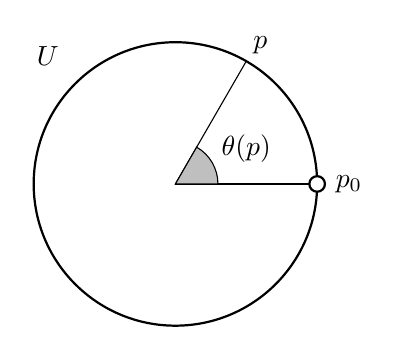
\begin{tikzpicture}[scale=0.9]
\draw[thick] (0,0) circle [radius=2];
\draw (0,0) -- (2,0);
\draw (0,0) -- (2*cos 60, 2* sin 60) node[above right=-1pt] {$p$};
\filldraw[fill=lightgray] (0,0) -- (0.6,0) arc (0:60:0.6) -- cycle;
\draw (1,0.5) node {$\theta(p)$};
\draw (-1.8,1.8) node {$U$};
\draw[thick,fill=white] (2,0) circle [radius=0.11] node[right=3pt] {$p_0$};
\end{tikzpicture}
\ese

\v

The operation:
\bse
p_1\bullet p_2 \coloneqq (\theta(p_1)+\theta(p_2))\! \mod 2\pi
\ese

endows $S^1\cong_{\mathrm{diff}}\SO(2,\R)$ with the structure of a Lie group. Then, a representation of $\SO(2,\R)$ is
given by:
\bi{rrCl}
R\cl & \SO(2,\R) & \to & \GL(\R^2)\\[5pt]
& p & \mapsto & \biggl( \begin{matrix} \cos \theta(p) & \sin \theta(p) \\ -\sin \theta (p) & \cos \theta(p)
\end{matrix}\biggr)
\ei

Indeed, the addition formula for sine and cosine imply that:
\bse
R(p_1\bullet p_2) = R(p_1)\circ R(p_2)
\ese
\ee

\be
Let $G$ be a Lie group (we suppress the $\bullet$ in this example). For each $g\in G$, define the Adjoint map:
\bi{rrCl}
\Ad_g \cl & G & \to & G\\ & h & \mapsto & g h g^{-1}
\ei

Note the capital ``A'' to distinguish this from the adjoint map on Lie algebras. Since $\Ad_g$ is a composition of
the Lie group multiplication and inverse map, it is a smooth map. Moreover, we have:
\bse
\Ad_g(e) = geg^{-1} = gg^{-1} = e
\ese

Hence, the push-forward of $\Ad_g$ at the identity is the map:
\bse
({\Ad_g}_*)_e \cl T_e G \xrightarrow{\sim} T_{\Ad_g(e)}G=T_e G
\ese

Thus, we have $\Ad_g\in\End(T_e G)$. In fact, you can check that:
\bse
({\Ad_{g^{-1}}}_*)_e\circ ({\Ad_g}_*)_e = ({\Ad_g}_*)_e \circ ({\Ad_{g^{-1}}}_*)_e = \id_{T_e G}
\ese

and hence, we have, in particular, $\Ad_g\in\GL(T_e G)\cong_{\mathrm{Lie\, grp}}\GL(\mathcal{L}(G))$ \v

\noindent We can therefore construct a map:
\bi{rrCl}
\Ad \cl & G & \to & \GL(T_e G)\\ & g & \mapsto & {\Ad_g}_*
\ei

which, as you can check, is a representation of $G$ on its Lie algebra.
\ee

Since a representation $R$ of a Lie group $G$ is required to be smooth, we can always consider its differential or
push-forward at the identity:
\bse
(R_*)_e \cl T_e G \xrightarrow{\sim} T_{\id_V}\!\GL(V)
\ese

Since for any $A,B\in T_e G$ we have:
\bse
(R_*)_e[A,B] =[(R_*)_eA,(R_*)_eB]
\ese

the map $(R_*)_e$ is a representation of the Lie algebra of $G$ on the vector space $\GL(V)$. In fact, in the
previous example we have:
\bse
(\Ad_*)_e = \ad
\ese

where $\ad$ is the adjoint representation of $T_e G$.

\section{Reconstruction Of A Lie group From Its Lie Algebra}

We have seen in detail how to construct a Lie algebra from a given Lie group. We would now like to consider the
inverse question, i.e.\ whether, given a Lie algebra, we can construct a Lie group whose associated Lie algebra is
the given one and, if this is the case, whether this correspondence is actually bijective. \v

We will find that the answer to the first question is affirmative. Given a Lie algebra, we will construct a Lie group
via something called the exponential map. However, we can already answer in the negative the second question, since
there examples of Lie groups which are not isomorphic but give rise to the same Lie algebra. Hence, the
correspondence between Lie groups and Lie algebras cannot be bijective. \v

Recall that in the chapter of topological manifolds we defined the integral curve $\gamma\cl(-\varepsilon, \varepsilon)
\to M$ on a smooth manifold $M$ as:
\bse
\forall \, \lambda \in (-\varepsilon,\varepsilon) : \ X_{\gamma,\gamma (\lambda)} = X(\gamma(\lambda))
\ese

\v

and based on that we defined a complete vector field as the vector field where the integral $(-\varepsilon,
\varepsilon)$ of $\gamma$ can be extended to the whole $R$ which from there followed that for any $p$ on $M$ it is $X
(p) = X_p$. \v

Finally, we gave a theorem that stated that on a compact manifold, every vector field is complete, and given that we
only work with compact manifolds we have been using the fact that $X(p) = X_p$. \v

However, on a Lie group, even if non-compact, there are always complete vector fields.

\bt[]
Every left-invariant vector field on a Lie group is complete.
\et

The integral curves of left-invariant vector fields are crucial in the construction of the map that allows us to go
from a Lie algebra to a Lie group.

\subsection{The Exponential Map}

Let $G$ be a Lie group. Recall that given any $X_e\in T_e G$, we can define the uniquely determined left-invariant
vector field $X \coloneqq j(A)$ via the isomorphism $j\cl T_e G \xrightarrow{\sim}\mathcal{L}(G)$ as:
\bse
X(g) = j(X_e)(g) \coloneqq (\ell_{g*})_e (X_e)
\ese

Then let $\gamma \cl \R \to G$ be the maximal integral curve of $X$ with $\gamma(0) = e\in G$.

\bd [Exponential Map]
Let $G$ be a Lie group. The \textbf{exponential map} is defined as:
\bi{rrCl}
\exp \cl & T_e G & \to & G\\ & X_e & \mapsto & \exp(X_e) \coloneqq \gamma(1)
\ei
\ed

\bt[]
\ben[label=\roman*)]
\item The map $\exp$ is smooth and a local diffeomorphism around $0\in T_e G$, i.e.\ there exists an open $V\se T_e G$
containing $0$ such that the restriction:
\bse
\exp|_V\cl V \to \exp(V) \se G
\ese

is bijective and both $\exp|_V$ and $(\exp|_V)^{-1}$ are smooth.
\item If $G$ is compact, then $\exp$ is surjective.
\een
\et

The first part of the theorem says that we can recover a neighbourhood of the identity of $G$ from a neighbourhood of
the identity of $T_e G$. \v

Since $T_e G$ is a vector space, it is non-compact (intuitively, it extends infinitely far away in every direction)
and hence, if $G$ is compact, $\exp$ cannot be injective. This is because, by the second part of the theorem, it
would then be a diffeomorphism $T_e G\to G$. But as $G$ is compact and $T_e G$ is not, they are not diffeomorphic.

\bt[]
Let $G$ be a Lie group. The image of $\exp\cl T_e G\to G$ is the connected component of $G$ containing the identity.
\et

Therefore, if $G$ itself is connected, then $\exp$ is again surjective. Note that, in general, there is no relation
between connected and compact topological spaces, i.e.\ a topological space can be either, both, or neither.

\be
Let $B\cl V\times V$ be a pseudo inner product on $V$. Then:
\bse
\Ort(V) \coloneqq \{\phi\in \GL(V)\mid \forall \, v,w\in V : B(\phi(v), \phi(w))=B(v,w)\}
\ese

is called the \emph{orthogonal group} of $V$ with respect to $B$. Of course, if $B$ or the base field of $V$ need to
be emphasized, they can be included in the notation. Every $\phi\in \Ort(V)$ has determinant $1$ or $-1$. Since the
determinant is multiplicative, we have a subgroup:
\bse
\SO(V) \coloneqq \{\phi\in \Ort(V)\mid \det\phi = 1\}
\ese

These are, in fact, Lie subgroups of $\GL(V)$. The Lie group $\SO(V)$ is connected while:
\bse
\Ort(V)=\SO(V)\cup \{\phi\in \Ort(V)\mid \det \phi = -1\}
\ese

is disconnected. Since $\SO(V)$ contains $\id_V$, we have:
\bse
\so(V) \coloneqq T_{\id_V}\!\SO(V) = T_{\id_V}\!\Ort(V) \eqqcolon \ort(V)
\ese

and:
\bse
\exp(\so(V))=\exp(\ort(V))=\SO(V)
\ese
\ee

Choosing a basis $X_1,\ldots,X_{\dim G}$ of $T_e G$ often provides a convenient co-ordinatisation of $G$ near $e$.
Consider, for example, the Lorentz group:
\bse
\Ort(3,1) \equiv \Ort(\R^4) = \{\Lambda\in \GL(\R^4)\mid \forall \, x,y\in \R^4 : B(\Lambda(x),\Lambda(y))=B(x,y) \}
\ese

where $B(x,y) \coloneqq \eta_{\mu\nu}x^\mu y^\nu$, with $0\leq \mu,\nu\leq 3$ and:
\bse
[\eta^{\mu\nu}] = [\eta_{\mu\nu}] \coloneqq \left(
\begin{matrix} -1 & 0 & 0 & 0 \\ 0 & 1 & 0 & 0 \\ 0 & 0 & 1 & 0 \\ 0 & 0 & 0 & 1 \end{matrix}\right)
\ese

The Lorentz group $\Ort(3,1)$ is $6$-dimensional, hence, so is the Lorentz algebra $\ort(3,1)$. We could simply denote
the basis of $\ort(3,1)$ as $\{X_i\mid i=1,\ldots,6\}$, but it is used to denote it as $\{M^{\mu\nu}\mid 0\leq \mu,
\nu\leq 3\}$ and require that the indices $\mu,\nu$ be antisymmetric, i.e.\ :
\bse
M^{\mu\nu} = -M^{\nu\mu }
\ese

Then $M^{\mu\nu}=0$ when $\rho=\sigma$, and the set $\{M^{\mu\nu}\mid 0\leq \mu,\nu\leq 3\}$, while technically not
linearly independent, contains the 6 independent elements that we want to consider as a basis. These basis elements
satisfy the following bracket relation:
\bse
[M^{\mu\nu},M^{\rho\sigma}] =\eta^{\nu\sigma} M^{\mu\rho} +\eta^{\mu\rho} M^{\nu\sigma} -\eta^{\nu\rho} M^{\mu\sigma}
-\eta^{\mu\sigma} M^{\nu\rho}
\ese

Any element $\lambda\in \ort(3,1)$ can be expressed as linear combination of the $M^{\mu\nu}$:
\bse
\lambda = \tfrac{1}{2}\omega_{\mu\nu}M^{\mu\nu}
\ese

where the indices on the coefficients $\omega_{\mu\nu}$ are also antisymmetric, and the factor of $\tfrac{1}{2}$
ensures that the sum over all $\mu,\nu$ counts each antisymmetric pair only once. Then, we can recover part of the
Lie Group $\Ort(3,1)$ by the use of the exponential map:
\bse
\Lambda = \exp(\lambda) = \exp(\tfrac{1}{2}\omega_{\mu\nu}M^{\mu\nu}) \in \Ort(3,1)
\ese

The subgroup of $\Ort(3,1)$ consisting of the the space-orientation preserving Lorentz transformations, or
\emph{proper} Lorentz transformations, is denoted by $\SO(3,1)$. The subgroup consisting of the time-orientation
preserving, or \emph{orthochronous}, Lorentz transformations is denoted by $\Ort^+(3,1)$. The Lie group $\Ort(3,1)$
is disconnected. Its four connected components are:
\ben[label=\roman*)]
\item $\SO^+(3,1) \coloneqq \SO(3,1)\cap\Ort^+(3,1)$, also called the \emph{restricted Lorentz group}, consisting of
the proper orthochronous Lorentz transformations.
\item $\SO(3,1)\sm \Ort^+(3,1)$, the proper non-orthochronous transformations.
\item $\Ort^+(3,1)\sm\SO(3,1)$, the improper orthochronous transformations.
\item $\Ort(3,1)\sm (\SO(3,1)\cup\Ort^+(3,1))$, the improper non-orthochronous transformations.
\een

Since $\id_{\R^4}\in \SO^+(3,1)$, we have $\exp(\ort(3,1))=\SO^+(3,1)$. Then $\{M^{\mu\nu}\}$ provides a nice
co-ordinatisation of $\SO^+(3,1)$ since, if we choose:

\bse
[\omega_{\mu\nu}] = \left( \begin{matrix}
0 & \psi_1 & \psi_2 & \psi_3 \\
-\psi_1 & 0 & \varphi_3 & -\varphi_2 \\
-\psi_2 & -\varphi_3 & 0 & \varphi_1 \\
-\psi_3 & \varphi_2 & -\varphi_1 & 0
\end{matrix} \right)
\ese

then the Lorentz transformation $\exp(\tfrac{1}{2}\omega_{\mu\nu}M^{\mu\nu}) \in \SO^+(3,1)$ corresponds to a boost
in the $(\psi_1,\psi_2,\psi_3)$ direction and a space rotation by $(\varphi_1, \varphi_2,\varphi_3)$. Indeed, in
physics one often thinks of the Lie group $\SO^+(3,1)$ as being generated by $\{M^{\mu\nu}\}$. \v

A representation $\rho\cl T_{\id_{\R^4}}\!\SO^+(3,1)\xrightarrow{\sim} \End (\R^4)$ is given by:
\bse
\rho(M^{\mu\nu})^a_{\phantom{a}b} \coloneqq \eta^{\nu a}\delta^{\mu}_b - \eta^{\mu a}\delta^{\nu}_b
\ese

which is probably how you have seen the $M^{\mu\nu}$ themselves defined in physics courses. Using this
representation, we get a corresponding representation:
\bi{rrCl}
R\cl & \SO^+(3,1) \to \GL(\R^4)
\ei

via the exponential map by defining:
\bse
R(\Lambda) = \exp(\tfrac{1}{2}\omega_{\mu\nu}\rho(M^{\mu\nu}))
\ese

Then, the map $\exp$ becomes the usual exponential (series) of matrices.

\bd [One-Parameter Subgroup]
A \textbf{one-parameter subgroup} of a Lie group $G$ is a Lie group homomorphism:
\bse
\xi \cl \R \to G
\ese

with $\R$ understood as a Lie group under ordinary addition.
\ed

\be
Let $M$ be a smooth manifold and let $X\in\Gamma(TM)$ be a complete vector field. The \emph{flow} of $X$ is the
smooth map:
\bi{rrCl}
\Theta \cl & \R\times M & \to & M\\ & (\lambda,p) & \mapsto & \Theta_\lambda(p) \coloneqq \gamma_p(\lambda)
\ei

where $\lambda_p$ is the maximal integral curve of $X$ through $p$. For a fixed $p$, we have:
\bse
\Theta_{0} = \id_M, \qquad \Theta_{\lambda_1}\circ \Theta_{\lambda_2} = \Theta_{\lambda_1+\lambda_2}, \qquad
\Theta_{-\lambda} = \Theta_{\lambda}^{-1}
\ese

For each $\lambda\in \R$, the map $\Theta_\lambda$ is a diffeomorphism $M\to M$. Denoting by $\mathrm{Diff}(M)$ the
group (under composition) of the diffeomorphisms $M\to M$, we have that the map:
\bi{rrCl}
\xi \cl & \R & \to & \mathrm{Diff}(M)\\ & \lambda & \mapsto & \Theta_\lambda
\ei

is a one-parameter subgroup of $\mathrm{Diff}(M)$.
\ee

\bt[]
Let $G$ be a Lie group.
\ben[label=\roman*)]
\item Let $X_e\in T_e G$. The map:
\bi{rrCl}
\xi^{X_e}\cl & \R & \to & G\\ & \lambda & \mapsto & \xi^{X_e}(\lambda) \coloneqq \exp(\lambda X_e)
\ei

is a one-parameter subgroup.
\item Every one-parameter subgroup of $G$ has the form $\xi^{X_e}$ for some $X_e\in T_e G$.
\een
\et

Therefore, the Lie algebra allows us to study all the one-parameter subgroups of the Lie group.

\bt[]
Let $G$ and $H$ be Lie groups and let $\phi\cl G \to H$ be a Lie group homomorphism. Then, for all $X_e\in T_{e}G$, we
have:
\bse
\phi (\exp (X_e))= \exp ((\phi_*)_{e} X_e)
\ese

Equivalently, the following diagram commutes:
\bse
\begin{tikzcd}
T_{e_G}G \ar[dd,"\exp"'] \ar[rr,"(\phi_*)_{e}"]&& T_{e_H}H\ar[dd,"\exp"]\\ &&\\ G\ar[rr,"\phi"] && H
\end{tikzcd}
\ese
\et

In particular, for $\phi\equiv \Ad_g\cl G\to G$, we have:
\bse
\Ad_g (\exp(X_e)) = \exp(({\Ad_g}_*)_e X_e)
\ese

\section{Lie Group Actions On A Manifold}

\bd [Left Lie Group Action]
Let $(G,\bullet)$ be a Lie group and let $M$ be a smooth manifold. A smooth map:
\bi{rrCl}
\lacts \cl & G\times M & \to & M\\ & (g,p) & \mapsto & g \lacts p
\ei

satisfying:
\ben[label=\roman*)]
\item $\forall \, p \in M :\ e\lacts p = p$.
\item $\forall \, g_1,g_2\in G : \forall \, p\in M : \ (g_1\bullet g_2) \lacts p = g_1 \lacts (g_2 \lacts p)$.
\een

is called a \textbf{left Lie group action}, or \textbf{left $G$-action}, on $M$.
\ed

\bd [Left $G$-Manifold]
A manifold equipped with a left $G$-action is called a \textbf{left $G$-manifold}.
\ed

Note that in the above definition, the smooth structures on $G$ and $M$ were only used in the requirement that 
$\lacts$ be smooth. By dropping this condition, we obtain the usual definition of a group action on a set. Some of 
the definitions that we will soon give for Lie groups and smooth manifolds, such as those of orbits and stabilisers, 
also have clear analogues to the case of bare groups and sets.

\be
Let $G$ be a Lie group and let $R\cl G \to \GL(V)$ be a representation of $G$ on a vector space $V$. Define a map:

\vspace{-20pt}

\bi{rrCl}
\lacts \cl & G \times V & \to & V\\ & (g,v) & \mapsto & g\lacts v \coloneqq R(g)v
\ei

We easily check that $e\lacts v \coloneqq R(e)v = \id_V v = v$ and:
\bi{rCl}
(g_1\bullet g_2) \lacts v & \coloneqq & R(g_1\bullet g_2)v\\
& = & (R(g_1)\circ R(g_2))v\\
& = & R(g_1)( R(g_2)v)\\
& = & g_1 \lacts (g_2 \lacts v)
\ei

for any $v\in V$ and any $g_1,g_2\in G$. Moreover, if we equip $V$ with the usual smooth structure, the map $\lacts$ 
is smooth and hence, a Lie group action on $V$. It follows that representations of Lie groups are just a special case
of left Lie group actions. We can therefore think of left $G$-actions as generalised representations of $G$ on some 
manifold. 
\ee

\bd [Right Lie Group Action]
Similarly, a \textbf{right Lie group action} or \textbf{right $G$-action} on $M$ is a smooth map:
\bi{rrCl}
\racts \cl & M\times G & \to & M\\ & (p,g) & \mapsto & p \racts g
\ei

satisfying:
\ben[label=\roman*)]
\item $\forall \, p \in M :\ p\racts g = p$.
\item $\forall \, g_1,g_2\in G : \forall \, p\in M : \ p \racts (g_1\bullet g_2) = (p \racts g_1) \racts g_2$.
\een
\ed

\bt[]
Let $\lacts$ be a left $G$-action on $M$. Then:
\bi{rrCl}
\racts \cl & M\times G & \to & M\\ & (p,g) & \mapsto & p \racts g \coloneqq g^{-1} \lacts p
\ei

is a right $G$-action on $M$.
\et

\bq
First note that $\racts$ is smooth since it is a composition of $\lacts$ and the inverse map on $G$, which are both 
smooth. We have $p\racts e \coloneqq e \lacts p = p$ and:
\bi{rCl}
p \racts (g_1\bullet g_2) & \coloneqq & (g_1\bullet g_2)^{-1} \lacts p\\[5pt]
& = & (g_2^{-1}\bullet g_1^{-1}) \lacts p\\[5pt]
& = & g_2^{-1} \lacts (g_1^{-1} \lacts p)\\[5pt]
& = & g_2^{-1} \lacts (p \racts g_1)\\[5pt]
& = & (p \vartriangleleft g_1) \vartriangleleft g_2
\ei

for all $p\in M$ and $g_1,g_2\in G$, and hence, $\racts$ is a right $G$-action.
\eq

Since for each $g\in G$ we also have $g^{-1}\in G$, if we need \emph{some} action of $G$ on $M$, then a left action 
is just as good as a right action. Only later, within the context of principal and associated fibre bundles, we will 
attach separate ``meanings'' to left and right actions. Some of the next definitions and results will only be given 
in terms of left actions, but they obviously apply to right actions as well. \v

Recall that if we have a basis $\{ e_1,\ldots,e_{\dim M} \}$ of $T_p M$ and $X^1,\ldots,X^{\dim M}$ are the 
components of some $X_p \in T_p M$ in this basis, then under a change of basis:

\bse
\widetilde e_a = A^b_{\phantom{b}a}e_b
\ese

we have $X=\widetilde X^a \widetilde e_a$, where:
\bse
\widetilde X^a = (A^{-1})^a_{\phantom{a}b}X^b
\ese

\v

Once expressed in terms of principal and associated fibre bundles, we will see that the ``recipe'' of labelling the 
basis by lower indices and the vector components by upper indices, as well as their transformation law, can be 
understood as a right action of $\GL(\dim M, \R)$ on the basis and a left action of the same $\GL(\dim M, \R)$ on the
components.

\bd [$\rho$-Equivariant Map]
Let $G,H$ be Lie groups, let $\rho\cl G\to H$ be a Lie group homomorphism and let:
\bi{l}
\lacts \cl G \times M \to M\\ \blacktriangleright \cl H \times N \to N
\ei

be left actions of $G$ and $H$ on some smooth manifolds $M$ and $N$, respectively. Then, a smooth map $f\cl M\to N$ 
is said to be \textbf{$\rho$-equivariant} if the diagram:

\bse
\adjustbox{scale=1.5,center}{
\begin{tikzcd}
G\times M \ar[dd,"\lacts"'] \ar[rr,"\rho\times f"]&& H\times N \ar[dd,"\blacktriangleright"]\\
&&\\
M \ar[rr,"f"] && N
\end{tikzcd}}
\ese

\v

where
\bse
(\rho\times f)(g,p) \coloneqq (\rho(g),f(p))\in H\times N
\ese

commutes. \v

Equivalently:
\bse
\forall \, g \in G : \forall \, p \in M : \ f(g\lacts p) = \rho(g) \blacktriangleright f(p)
\ese
\ed

In other words, if $\rho\cl G \to H$ is a Lie group homomorphism, then the $\rho$-equivariant maps are the 
``action-preserving'' maps between the $G$-manifold $M$ and the $H$-manifold $N$. \v

Note that by setting $\rho = \id_G$ or $f=\id_M$, the notion of $f$ being $\rho$-equivariant reduces to what we might
call a homomorphism of $G$-manifolds in the former case, and a homomorphism of left actions on $M$ in the latter.

\bd[Orbit]
Let $\lacts \cl G \times M \to M$ be a left $G$-action. For each $p\in M$, we define the \textbf{orbit} 
of $p$ as the set:
\bse
G_p \coloneqq \{q\in M\mid \exists \, g\in G : q = g\lacts p\}
\ese
\ed

Alternatively, the orbit of $p$ is the image of $G$ under the map $( {}-\lacts p)$. It consists of all the points in 
$M$ that can be reached from $p$ by successive applications of the action $\lacts$.

\be
Consider the action induced by representation of $\SO(2,\R)$ as rotation matrices in $\End(\R^2)$. The orbit of any 
$p\in\R^2$ is the circle of radius $|p|$ centred at the origin. \v

\begin{center}
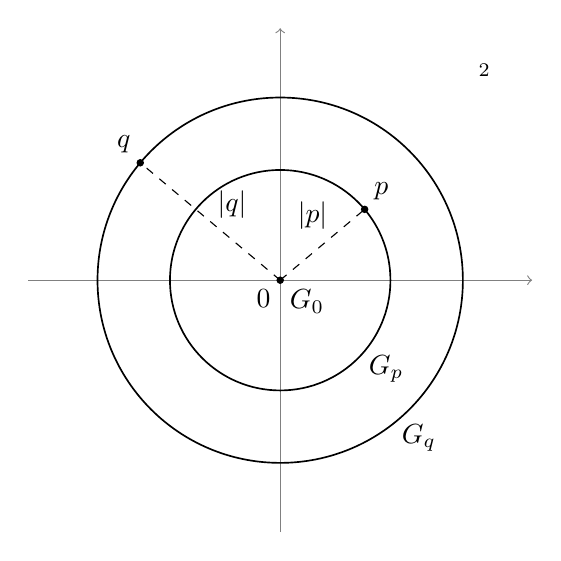
\begin{tikzpicture}[scale=0.8]
\draw[gray,->] (0,-4) -- (0,4);
\draw[gray,->] (-4,0) -- (4,0);
\draw (3.25,3.25) node {$\R^2$};
\draw[dashed] (0,0) -- (1.75*cos 40, 1.75*sin 40) node[above right] {$p$};
\draw[fill] (1.75*cos 40, 1.75*sin 40) circle[radius=0.05];
\draw (1.75*cos -40, 1.75*sin -40) node[below right=-2pt] {$G_p$};
\draw (-0.1+0.8*cos 40, 0.8*sin 40) node[above=3pt] {$|p|$};
\draw[dashed] (0,0) -- (2.9*cos 140, 2.9*sin 140) node[above left] {$q$};
\draw[fill] (2.9*cos 140, 2.9*sin 140) circle[radius=0.05];
\draw (2.9*cos -50, 2.9*sin -50) node[below right=-2pt] {$G_q$};
\draw(1*cos 140, 1*sin 140) node[above=4pt ] {$|q|$};
\draw[semithick] (0,0) circle [radius=1.75];
\draw[semithick] (0,0) circle [radius=2.9];
\draw[fill] (0,0) circle [radius=0.05] node[below right] {$G_0$};
\draw(0,0) node[below left] {$0$};
\end{tikzpicture}
\end{center}
\ee

\v

It should be intuitively clear from the definition that the orbits of two points are either disjoint or coincide. In 
fact, we have the following.

\bt[]
Let $\lacts \cl G\times M \to M$ be an action on $M$. Define a relation on $M$:
\bse
p\sim q \ :\Leftrightarrow \ \exists \, g \in G : q = g \lacts p
\ese

Then $\sim$ is an equivalence relation on $M$.
\et

\bq
Let $p,q,r\in M$. We have:
\ben
[label=\roman*)]
\item $p\sim p$ since $p = e \lacts p$.
\item $p\sim q \Rightarrow q\sim p$ since, if $q =g \lacts p$, then:
\bse
p = e \lacts p = (g^{-1}\bullet g) \lacts p = g^{-1}\lacts( g \lacts p)= g^{-1}\lacts q
\ese

\item $(p\sim q$ and $q\sim r) \Rightarrow p\sim r$ since, if $q =g_1 \lacts p$ and $r =g_2 \lacts q$, then:
\bse
r = g_2 \lacts (g_1 \lacts p) = (g_1\bullet g_2)\lacts p
\ese
\een

Therefore, $\sim$ is an equivalence relation on $M$.
\eq

The equivalence classes of $\sim$ are, by definition, the orbits.

\bd [Orbit Space]
Let $\lacts\cl G\times M\to M$ be an action on $M$. The \textbf{orbit space} of $M$ is:
\bse
M/G \coloneqq M/\!\sim \,= \{G_p \mid p\in M\}
\ese
\ed

\be
The orbit space of our previous $\SO(2,\R)$-action on $\R^2$ is the partition of $\R^2$ into concentric circles 
centred at the origin, plus the origin itself. 
\ee

\bd [Stabiliser]
Let $\lacts\cl G\times M\to M$ be a $G$-action on $M$. The \textbf{stabiliser} of $p\in M$ is:
\bse
S_p \coloneqq \{g\in G\mid g\lacts p = p\}
\ese
\ed

Note that for each $p\in M$, the stabiliser $S_p$ is a subgroup of $G$.
\be
In our $\SO(2,\R)$ example, we have $S_p=\{\id_{\R^2}\}$ for $p\neq 0$ and $S_0=\SO(2,\R)$.
\ee

\bd [Free / Transitive Actions]
A left $G$-action $\lacts\cl G\times M\to M$ is said to be:
\ben[label=\roman*)]
\item \textbf{Free} if for all $p\in M$, we have $S_p=\{e\}$.
\item \textbf{Transitive} if for all $p,q\in M$, there exists $g\in G$ such that $p=g\lacts p$.
\een
\ed

\be
The action $\lacts\cl G\times V \to V$ induced by a representation $R\cl G\to \GL(V)$ is never free since $\GL(V)$ 
contains all the invertible linear transformation which, by definition, map $0$ to $0$ hence, we always have $S_0=G$.
\ee

\be
Consider the action $\lacts\cl \mathrm{T}(n)\times \R^n\to \R^n$ of the $n$-dimensional translation group $\mathrm{T}
(n)$ on $\R^n$. We have, rather trivially, $\mathrm{T}(n)_p=\R^n$ for every $p\in \R^n$.It is also easy to show that 
this action is free and transitive. 
\ee

\bt[]
Let $\lacts\cl G \times M \to M$ be a free action. Then:
\bse
g_1 \lacts p = g_2 \lacts p \quad \Leftrightarrow \quad g_1 = g_2
\ese
\et

\bq
The $(\Leftarrow)$ direction is obvious. Suppose that there exist $p\in M$ and $g_1,g_2\in G$ such that $g_1 \lacts p
= g_2 \lacts p$. Then:
\bi{rCl}
g_1 \lacts p = g_2 \lacts p &\quad \Leftrightarrow \quad & g_2^{-1} \lacts 
(g_1 \lacts p) = g_2^{-1} \lacts(g_2 \lacts p)\\[5pt]
& \Leftrightarrow & (g_2^{-1} \bullet g_1) \lacts p = (g_2^{-1}\bullet g_2) \lacts p\\[5pt]
& \Leftrightarrow & (g_2^{-1}\bullet g_1) \lacts p = (e\lacts p)\\[5pt]
& \Leftrightarrow & (g_2^{-1}\bullet g_1) \lacts p = p
\ei

Hence, $g_2^{-1}\bullet g_1\in S_p$, but since $\lacts$ is free we have $S_p=\{e\}$, and thus $g_1=g_2$.
\eq

\bt[]
If $\lacts\cl G \times M \to M$ is a free action, then:
\bse
\forall \, p \in G :\ G_p \cong_{\mathrm{diff}} G
\ese
\et

\be
Define $\lacts\cl \SO(2,\R)\times \R^2\sm\{0\}\to \R^2\sm\{0\}$ to coincide with the action induced by the 
representation of $\SO(2,\R^2)$ on $\R^2$ for each non-zero point of $\R^2$. Then this action is free, since we have 
$S_p=\{\id_{\R^2}\}$ for $p\neq 0$, and the previous proposition implies:

\bse
\forall \, p\in \R^2\sm\{0\} : \ \SO(2,\R)_p \cong_{\mathrm{diff}} \SO(2,\R) \cong_{\mathrm{diff}} S^1
\ese
\ee